\documentclass{article}

% Official ICLR 2026 style and bibliography format from the prior COMPOSE submission.
\usepackage{iclr2026_conference,times}
\usepackage[utf8]{inputenc}
\usepackage[T1]{fontenc}
\usepackage{microtype}
\usepackage{amsmath,amssymb,mathtools,bm}
\usepackage{amsthm}
\usepackage{booktabs,tabularx,array}
\usepackage{xspace}
\usepackage{float}
\usepackage{graphicx}
\usepackage{xcolor}
\usepackage{enumitem}
\usepackage{pifont}
\usepackage{url}
\usepackage{hyperref}
\usepackage[capitalize,noabbrev]{cleveref}

\hypersetup{colorlinks=true,citecolor=blue!55!black,linkcolor=blue!55!black,urlcolor=blue!55!black}
% Centralized placeholders for the control-substrate reframe.
%
% FRAMING-ONLY DRAFT (2026-07-22 author override): EVERY numerical *result* is \XXX,
% including results we already have committed artifacts for (barrier-mechanism
% percentages, structural-control satisfaction rates, oracle efficiency, the Doob
% endpoint error, de-novo validity/uniqueness/diversity, etc.). Numbers may still move
% after the source-conditioned (Stage B) and ring-fix retrains, so nothing is committed
% here. Each macro's comment says exactly what result belongs there and where the frozen
% artifact lives, so the value can be dropped in later without touching prose. Only
% non-result design hyperparameters (N_max, width, depth, lr, schedule) are kept as real
% numbers, and those live inline in the method/appendix, not here.
\newcommand{\XXX}{\textcolor{red}{XXX}}

% ---------------------------------------------------------------------------
% De novo sufficiency (GuacaMol C/N/O/F base). Validity and all-step validity/
% connectivity are 100% BY CONSTRUCTION (Prop. closure); we nonetheless leave the
% reported *rate* as \XXX pending the frozen multi-seed run. Uniqueness / novelty /
% internal diversity / descriptor distances / coverage are all \XXX; the ring-taxonomy
% defect means the final numbers await the ring-fix at-scale retrain.
% ---------------------------------------------------------------------------
\newcommand{\ComposeValidity}{\XXX}
\newcommand{\ComposeTrajectoryValidity}{\XXX}
\newcommand{\ComposeTrajectoryConnectivity}{\XXX}
\newcommand{\ComposeUniqueness}{\XXX}
\newcommand{\ComposeNovelty}{\XXX}
\newcommand{\ComposeDescriptorW}{\XXX}
\newcommand{\ComposeDiversity}{\XXX}
\newcommand{\ComposeCoverage}{\XXX}
\newcommand{\ComposeMeanEvents}{\XXX}
\newcommand{\ComposeThroughput}{\XXX}
% FCD / GuacaMol KL deferred to the final GuacaMol table; not a headline here.
\newcommand{\ComposeFCD}{\XXX}
\newcommand{\ComposeKL}{\XXX}

% De-novo ring-taxonomy defect (honest partial; the mechanism-proven fix is untrained).
\newcommand{\DenovoSmallRing}{\XXX}       % small-ring (3--4) fraction, ring-defective base
\newcommand{\DenovoSmallRingRef}{\XXX}    % reference small-ring fraction
\newcommand{\DenovoAromatic}{\XXX}        % aromatic-atom fraction, base
\newcommand{\DenovoAromaticRef}{\XXX}     % reference aromatic-atom fraction

% Soft property steering (de-novo, controller Psi only): a demonstration of the control
% law's preference knob, NOT a sample-efficiency leaderboard entry.
\newcommand{\DenovoQEDRaw}{\XXX}          % raw de-novo mean QED
\newcommand{\DenovoQEDControlled}{\XXX}   % mean best QED under a QED-tilted controller
\newcommand{\DenovoQEDSuccess}{\XXX}      % QED success rate under control
\newcommand{\DenovoLogpDialErr}{\XXX}     % median |generated logP - target| across the dial

% Structural distribution metrics.
\newcommand{\ComposeSizeTV}{\XXX}
\newcommand{\ComposeCycleRankTV}{\XXX}
\newcommand{\ComposeRingSizeTV}{\XXX}
\newcommand{\ComposeElementTV}{\XXX}
\newcommand{\ComposeBondTV}{\XXX}

% Operator and coupling diagnostics.
\newcommand{\ComposeGraftFraction}{\XXX}
\newcommand{\ComposeGrowFraction}{\XXX}
\newcommand{\ComposeShrinkFraction}{\XXX}
\newcommand{\ComposeRetypeFraction}{\XXX}
\newcommand{\ComposeRingFraction}{\XXX}
\newcommand{\ComposePathLength}{\XXX}
\newcommand{\ComposeCatalogCoverage}{\XXX}

% Ablations.
\newcommand{\NullPriorFCD}{\XXX}
\newcommand{\PrimitiveTreeFCD}{\XXX}
\newcommand{\GraftTreeFCD}{\XXX}
\newcommand{\NoMacroFCD}{\XXX}
\newcommand{\NoAliasFCD}{\XXX}
\newcommand{\NoStratificationFCD}{\XXX}

% ---------------------------------------------------------------------------
% Mechanistic spotlight: Pareto reachability depends on path topology.
% Exact enumerated rewrite graphs; frozen artifacts in
% diagnostics/reachability/{pareto_reachability_cap4,pareto_reachability_cap5,
% frontier_recovery_cap4}.json (mean over 6 sources). All \XXX in this draft.
% ---------------------------------------------------------------------------
\newcommand{\ReachStatesCapFour}{\XXX}          % enumerated states, cap-4 graph
\newcommand{\ReachEdgesCapFour}{\XXX}           % enumerated edges, cap-4 graph
\newcommand{\ReachStatesCapFive}{\XXX}          % enumerated states, cap-5 graph
\newcommand{\BarrierSuboptTwoObj}{\XXX}         % cap-4, 2-obj: frac preference dirs monotone-suboptimal (mean)
\newcommand{\BarrierSuboptThreeObj}{\XXX}       % cap-4, 3-obj (mean)
\newcommand{\BarrierSuboptWorstTwoObj}{\XXX}    % cap-4, 2-obj: worst single source
\newcommand{\BarrierSuboptWorstThreeObj}{\XXX}  % cap-4, 3-obj: worst single source
\newcommand{\BarrierForfeitMean}{\XXX}          % mean fraction of reachable improvement forfeited when suboptimal
\newcommand{\BarrierForfeitMax}{\XXX}           % max (strict local maximum)
\newcommand{\BarrierInterior}{\XXX}             % interior-state incidence (size-cap-artifact control)
\newcommand{\BarrierBoundary}{\XXX}             % boundary-state incidence
\newcommand{\BarrierLookaheadTwo}{\XXX}         % cap-4, 2-obj: incidence under 2-edit evaluation lookahead
\newcommand{\BarrierLookaheadThree}{\XXX}       % cap-4, 2-obj: 3-edit lookahead
\newcommand{\BarrierSuboptCapFive}{\XXX}        % cap-5, 2-obj (mean)
\newcommand{\BarrierSuboptWorstCapFive}{\XXX}   % cap-5, 2-obj: worst single source
\newcommand{\BarrierForfeitCapFive}{\XXX}       % cap-5 mean forfeit
% Frontier recovery (exact): greedy structural ceiling vs detour-capable control.
% NOTE: recovery *efficiency* (matched-budget) is UNDECIDED -> stays \XXX by design.
\newcommand{\GreedyCoverageTwoObj}{\XXX}        % greedy frontier coverage ceiling, 2-obj
\newcommand{\GreedyHVTwoObj}{\XXX}              % greedy hypervolume fraction, 2-obj
\newcommand{\GreedyCoverageThreeObj}{\XXX}      % greedy frontier coverage ceiling, 3-obj
\newcommand{\DetourCoverageFull}{\XXX}          % detour-capable coverage at (unbounded) budget

% ---------------------------------------------------------------------------
% Structural control (hard constraints in the legal fiber vs generate-then-filter).
% Frozen CNOF-lead artifacts; all \XXX in this draft.
% ---------------------------------------------------------------------------
\newcommand{\ComposeScaffoldSatisfaction}{\XXX}      % in-fiber fixed-scaffold satisfaction
\newcommand{\ComposeSubstructureSatisfaction}{\XXX}  % required/forbidden SMARTS satisfaction
\newcommand{\ComposeScaffoldRetention}{\XXX}
\newcommand{\ComposeBaselineScaffoldEasy}{\XXX}      % gen-then-filter usable, small scaffolds
\newcommand{\ComposeBaselineScaffoldHard}{\XXX}      % gen-then-filter usable, largest scaffolds
\newcommand{\ComposeOracleEfficiency}{\XXX}          % oracle calls landing on feasible candidates
\newcommand{\ComposeBaselineOracleEfficiency}{\XXX}  % gen-then-filter oracle efficiency
\newcommand{\ComposeBaselineOracleWastedHard}{\XXX}  % wasted budget on hard scaffolds
\newcommand{\PhyschemBoxInFiber}{\XXX}               % per-sample: scaffold AND physchem box (COMPOSE)
\newcommand{\PhyschemBoxBaseline}{\XXX}              % per-sample: scaffold AND physchem box (gen-then-filter)
\newcommand{\PhyschemBoxFactor}{\XXX}                % per-sample advantage factor
\newcommand{\ConjunctionFullSpec}{\XXX}              % gen-then-filter usable yield at full conjoined spec

% Constrained optimization / anytime behaviour.
\newcommand{\ComposeConstrainedQEDFrom}{\XXX}
\newcommand{\ComposeConstrainedQEDTo}{\XXX}
\newcommand{\ComposeConstrainedQEDGain}{\XXX}
\newcommand{\ComposeConstrainedLeadsImproved}{\XXX}
\newcommand{\ComposeAnytimeCalls}{\XXX}              % median lead: oracle calls to 90% of final gain
\newcommand{\ComposePropertyGain}{\ComposeConstrainedQEDGain}
\newcommand{\ComposeConditionalSuccess}{\XXX}        % de-emphasised unconstrained oracle-hungry success rate

% Exactness anchor (Doob h-transform on an exact enumerated CTMC slice).
\newcommand{\ComposeExactnessStates}{\XXX}           % enumerated states of the exact slice
\newcommand{\ComposeExactnessLinf}{\XXX}             % endpoint L-infinity error vs exact Bayes conditional
\newcommand{\ExactHParticleFactor}{\XXX}             % particle saving of exact-h twist vs untwisted SMC

% ---------------------------------------------------------------------------
% Anytime Pareto editing (the designed hero): FUTURE / needs the source-conditioned
% Stage B retrain. Every metric here is \XXX by design, not merely pending a freeze.
% ---------------------------------------------------------------------------
\newcommand{\EditFeasibleHV}{\XXX}          % feasible hypervolume AUC vs oracle calls
\newcommand{\EditUniqueND}{\XXX}            % unique nondominated molecules in the archive
\newcommand{\EditFrontierCoverage}{\XXX}    % source-relative frontier coverage
\newcommand{\EditSourceDistance}{\XXX}      % median source edit distance
\newcommand{\EditRetention}{\XXX}           % protected-structure retention
\newcommand{\EditLearnedVsUniform}{\XXX}    % learned-quotient vs uniform-legal proposal efficiency

% Reproducibility (design specs; kept out of the results but still \XXX in this draft).
\newcommand{\ComposeParameters}{\XXX}
\newcommand{\ComposeTrainHours}{\XXX}
\newcommand{\ComposePeakMemory}{\XXX}


\newcommand{\method}{\textsc{Compose}\xspace}
\newcommand{\rgm}{\textsc{RGM}\xspace}
\newcommand{\M}{\mathcal{M}_{\Gamma}}
\newcommand{\Rset}{\mathcal{R}}
\newcommand{\A}{\mathcal{A}}
\newcommand{\Sset}{\mathcal{S}}
\newcommand{\Z}{\mathcal{Z}}
\newcommand{\pdata}{p_{\mathrm{data}}}
\newcommand{\pzero}{\pi_0}
\newcommand{\T}{\mathsf{T}}
\newcommand{\legal}{\mathsf{Legal}}
\newcommand{\Match}{\mathsf{Match}}
\newcommand{\cmark}{\ding{51}}
\newcommand{\xmark}{\ding{55}}
\newcommand{\partialmark}{\ensuremath{\triangle}}
\newcommand{\E}{\mathbb{E}}
\newcommand{\R}{\mathbb{R}}
\newcommand{\one}{\mathbf{1}}
\newcolumntype{Y}{>{\raggedright\arraybackslash}X}

\newtheorem{theorem}{Theorem}
\newtheorem{proposition}[theorem]{Proposition}
\newtheorem{lemma}[theorem]{Lemma}
\newtheorem{corollary}[theorem]{Corollary}
\theoremstyle{definition}
\newtheorem{definition}[theorem]{Definition}
\newtheorem{assumption}[theorem]{Assumption}
\theoremstyle{remark}
\newtheorem{remark}[theorem]{Remark}
\crefname{assumption}{assumption}{assumptions}
\Crefname{assumption}{Assumption}{Assumptions}

\title{\method: Control-Closed Molecular Generation on Valid Rewrite Paths}
\author{Anonymous Authors}
\date{}
% \iclrfinalcopy

\begin{document}
\maketitle

\begin{abstract}
Most molecular generators learn a distribution over endpoints while their intermediate states are latent numerical objects, so any source-conditioned control---hard requirements, property preferences, editing---must be attached through noisy-state predictors, repair, or terminal filtering. We instead learn a single object: a stochastic process whose states are complete molecular graphs, whose transitions are executable rewrites (grow, shrink, retype, bond, subtree graft, ring), and whose probabilities live on \emph{canonical molecular successors} rather than syntactic action descriptions. Generator Matching recovers its marginal firing rates from certified endpoint-conditioned rewrite programs; we call the construction \emph{Rewrite Generator Matching} (\rgm) and its molecular instantiation \method. Because every committed state is a molecule, the process is \emph{closed under control}: any sampler that only deletes or reweights legal molecular transitions inherits molecular-state validity. This yields a one-line control law, $\widetilde Q_t(G,H)=\one\{C(H)\}\,Q_{\theta,t}(G,H)\,\Psi_t(G,H,\omega)$, where $\one\{C\}$ is hard support, $Q_{\theta}$ the learned quotient rate over canonical successors, and $\Psi$ an arbitrary controller (preference tilt, Doob $h$-transform, SMC, MH); de novo generation is $C\equiv1,\Psi\equiv1$ and source-conditioned editing sets $G_0=G_s$. Our empirical spotlight is a property of this substrate that is \emph{undefined} when intermediates are not molecules: \emph{Pareto reachability depends on path topology}. On exact enumerated rewrite graphs, greedy/monotone control is provably suboptimal for \BarrierSuboptTwoObj{} (two-objective) of preference directions and plateaus at a structural ceiling (\GreedyCoverageTwoObj{} frontier coverage) below the reachable Pareto frontier; barrier-gated molecules are reachable only through \emph{valid downhill detours}, which reach \DetourCoverageFull{} coverage. Supporting evidence shows hard constraints enforced in the legal fiber (fixed scaffold and required/forbidden motifs at \ComposeScaffoldSatisfaction{}) where a matched generate-then-filter baseline collapses (to \ComposeBaselineScaffoldHard{}), every oracle call spent on a feasible candidate (\ComposeOracleEfficiency{} vs \ComposeBaselineOracleEfficiency{}), and a Doob $h$-transform that reproduces the exact conditional to \ComposeExactnessLinf{}. As a \emph{de novo} generator the base is valid, unique, novel, and diverse but has a known ring-taxonomy defect (small rings \DenovoSmallRing{} vs reference \DenovoSmallRingRef{}); the mechanism-proven fix awaits an at-scale retrain, so we do not claim de novo state of the art. The substrate is designed for \emph{anytime Pareto-set editing}---every visited molecule is potential output in a source-relative nondominated archive---which we present as a designed capability and motivated future direction, not a completed result. Simple baselines (graph genetic algorithms, PMO) are strong; our claim is the substrate and its path-topology mechanism, not beating them at optimization.
\end{abstract}

\section{Introduction}

Molecular generative modeling is increasingly a control problem. Unconditional generation must reproduce a molecular distribution; property targeting and optimization must move probability toward desired regions of chemical space; editing must preserve specified structure while revising the rest. These are usually treated as separate models---one for $p(G)$, another for $p(G\mid c)$ with $c$ a property vector, scaffold, or source molecule. We argue they are consequences of a single object. Most generators learn a distribution over \emph{endpoints} while their intermediate states are latent numerical tensors, so any source-conditioned control must be attached after the fact through noisy-state predictors, repair, or terminal filtering, and any state consumed by a property oracle, hard constraint, or human-interpretable edit is not yet a molecule. Terminal sanitization cannot make an earlier oracle query chemically meaningful. Our starting point is the opposite discipline: keep the generative trajectory inside molecular space, so that the trajectory itself becomes the design object and controllers act on molecules rather than on encodings.

Graph diffusion and flow models have substantially advanced molecular distribution learning \citep{jo2022gdss,vignac2023digress,jo2023grum,xu2024disco,siraudin2024cometh,qin2025defog}. Their node, edge, and coordinate processes are expressive, but generally evolve in an ambient graph space whose intermediate states need not be connected or valence-admissible. GrIDDD, Edit Flows, and Morph extend this paradigm with insertion, deletion, or substitution, establishing flexible cardinality within learned generative dynamics \citep{ninniri2025griddd,havasi2025editflows,franke2026morph}. A complementary line makes constraints structural: ConStruct restricts graph diffusion, molecular grammars generate through legal productions, CoCoGraph performs validity-preserving swaps, and reaction-based GFlowNets traverse executable synthesis or editing transformations \citep{madeira2024construct,kajino2019mhg,guo2022grammar,ruizbotella2026cocograph,koziarski2024rgfn,zhu2026spacegfn}. These are important precedents rather than isolated ingredients to be claimed anew. We are unaware, however, of a Generator-Matched probability path from a directly samplable molecular prior to a data distribution whose learned transitions are simultaneously flexible-size, non-monotone, and closed over complete molecular states.

We obtain such a path by making the interface between two established theories explicit and operational for de novo molecular generation. Stochastic graph rewriting defines qualitative rules, their concrete matches and application conditions, and the CTMC semantics induced by match propensities \citep{danos2015thermodynamic,behr2021rewriting}. Generator Matching provides a regression principle for recovering a marginal infinitesimal generator from tractable conditional generators \citep{holderrieth2025generator}. The former does not explain how to learn a source-to-data generative transport, and the latter does not choose a molecular state space, executable event vocabulary, or chemistry-closed transition relation. We formulate \emph{Rewrite Generator Matching} (\rgm) to supply those objects: endpoint-conditioned executable rewrite programs define conditional generators, and Generator Matching learns their time- and context-dependent marginal firing rates on the rewrite state graph. Thus, established tools produce a new generative construction rather than a validity mask attached to an ambient graph process.

Our molecular realization is \method---\textbf{COM}positional \textbf{P}robabilistic \textbf{O}perator \textbf{S}ampling and \textbf{E}diting. A state is a complete, connected graph admitted by a declared 2D atom/bond/charge/implicit-hydrogen grammar. A typed rewrite at a concrete match is a marked jump; application conditions define its state-dependent legal support. Multiple marks can name the same chemical transition because of graph symmetries or alternative executable lowerings, so their rates are aggregated at the canonical molecular successor. This quotient is correctness machinery with precedent in stochastic rewriting and symmetry-aware graph generation, not a separate novelty claim. The important consequence is operational: probability evolves between molecules by executing rules, rather than between unconstrained atom--edge tensors by later interpreting or repairing them.

Training begins with a target-independent, degree-bounded carbon tree $G_0\sim\pzero$ and a data molecule $G_1\sim\pdata$. A randomized compiler produces a certified source-to-target rewrite program, and a progress CTMC on that program supplies the conditional rates required by Generator Matching. Marginalizing the target, coupling, program, and progress state yields a generator on observed molecular states, following the conditional-to-marginal and latent-process principles of Generator Matching \citep{holderrieth2025generator,billera2026latent}. The compiler is supervision, not a decoder. At inference, a fresh source is transformed by ancestral sampling from the learned CTMC without access to a target, trace, candidate bank, beam search, or terminal repair.

The choice of rewrite paths is also an inductive bias. A purely local compiler can technically correct size, labels, bonds, and topology, yet do so through long or ambiguous programs: a mismatched tree may be pruned and regrown, and a ring system may require tightly coordinated local events. We therefore retain general grow, shrink, retype, and bond rewrites while introducing two verified derived actions. \emph{Subtree Graft} moves a bridge-attached component and reconnects it atomically, revising global topology without exposing a disconnected state. \emph{Whole-ring-system rewrites} coordinate the growth or deletion of supported monocyclic, fused, bridged, spiro, aromatic, and non-aromatic systems. Each derived action has validity-checked primitive lowering and inverse semantics. They compress difficult paths within a universal edit substrate; they do not turn \method into a fragment vocabulary.

\paragraph{Closure under control.}
The payoff of staying in molecular space is a clean separation of concerns. Because every committed state is a molecule and the legal fiber $\A(G)$ already enumerates valid successors, \emph{any} sampler that only deletes or reweights those transitions remains in the molecular state space. Writing $\one\{C(H)\}$ for a hard support mask, $Q_{\theta,t}(G,H)$ for the learned quotient rate over canonical successors, and $\Psi_t$ for a controller, controlled generation is the one-line law
\begin{equation}
\widetilde Q_t(G,H)=\one\{C(H)\}\,Q_{\theta,t}(G,H)\,\Psi_t(G,H,\omega),\qquad H\neq G,
\label{eq:control-law}
\end{equation}
with the diagonal set to the negative outgoing rate. This single expression subsumes hard requirements ($\one\{C\}$), preference tilting ($\Psi=\exp\{\beta\,R(\Delta s(G,H)\cdot\omega)\}$), Doob control ($\Psi=h_t(H)/h_t(G)$), source-conditioned editing ($G_0=G_s$), dynamic preferences (time-varying $\omega_t$), and plain generation ($C\equiv1,\Psi\equiv1$). The controller is swapped without retraining and cannot leave $\M$ (\cref{prop:control-closure}). We call this closure under control, and it is the paper's umbrella contribution: \emph{control-closed molecular probability paths}.

\paragraph{What every-step validity buys.}
The litmus test for the framing is what becomes \emph{undefined}---not merely worse---if intermediate states were not molecules. Our sharpest instance is a path-topology phenomenon that we make the empirical spotlight: on the exact rewrite graph, greedy or monotone control has a structural ceiling below the reachable Pareto frontier, and the barrier-gated remainder is reachable only through \emph{valid downhill detours}---a statement with no meaning unless every intermediate is itself a scorable molecule. A second consequence is that the substrate is a native interface for \emph{anytime Pareto-set editing}: every visited molecule can enter a source-relative nondominated archive, seed a branch, or be reused under a new preference. We develop this as the framework's designed capability but flag it as future work---a fair editing result needs a source-conditioned model, and the present base is a de novo generator. Hard structural constraints are then one especially clean use of $\one\{C\}$, not the identity of the paper.

Our contributions are:
\begin{itemize}[leftmargin=*]
    \item \textbf{Control-closed molecular probability paths (umbrella).} We formulate Generator Matching over executable stochastic rewrite systems---\emph{Rewrite Generator Matching}---so that probability evolves on canonical molecular successors, and prove closure under the control law~\eqref{eq:control-law}: hard support, preference, Doob, SMC, and MH controllers reweight the same molecular rates without retraining and cannot leave the declared state space. To our knowledge this is the first instantiation of Generator Matching on a formal, chemistry-closed stochastic graph-rewrite system with a sampler-agnostic control interface.
    \item \textbf{Pareto reachability depends on path topology (mechanistic spotlight).} We define an objective barrier on the legal edit graph and show, on exact enumerated rewrite graphs, that greedy/monotone control is provably suboptimal for a substantial fraction of preference directions and plateaus below the reachable frontier, whereas nonmyopic valid-path control crosses the barrier through molecular detours. This phenomenon is only expressible because intermediates are molecules.
    \item \textbf{Structural control and an exactness foundation (supporting).} Hard scaffold and required/forbidden-motif constraints are enforced in the legal fiber where a matched generate-then-filter baseline collapses with constraint hardness; feasibility-before-scoring makes every oracle call land on a feasible candidate; and on a tractable exhaustive-state slice the Doob $h$-transform reproduces the exact conditional to machine precision.
    \item \textbf{A flexible-size molecular realization and its honest limits.} \method combines general grow/shrink/retype/bond rewrites with verified subtree-Graft and whole-ring-system operators, every committed state connected and grammar-valid. As a de novo generator it is valid, unique, novel, and diverse but has a known ring-taxonomy defect whose fix is mechanism-proven yet untrained at scale; the anytime-Pareto-editing hero and the learned-vs-uniform efficiency study run on the source-conditioned edit flow (\cref{sec:source-conditioned}), whose at-scale training is future work.
\end{itemize}

\begin{figure}[H]
\centering
\fbox{\begin{minipage}{0.95\linewidth}
\centering
\textbf{Training}\qquad
$G_0\sim\pzero,\;G_1\sim\pdata$
$\xrightarrow{\text{couple + compile}}$
$z=(G_0\xrightarrow{a_1}\cdots\xrightarrow{a_K}G_1)$

\vspace{5pt}
$z\xrightarrow{\text{sample }(t,k)}$
$(G_k,t,\;q_t^z)$
$\xrightarrow{\text{Generator Matching}}$
$q_\theta(a\mid G_k,t)$

\vspace{5pt}
\textbf{Inference}\qquad
$\widetilde G_0\sim\pzero$
$\xrightarrow[\text{no endpoint; no compiler; no beam}]{\text{ancestral learned rewrite CTMC}}$
$\widetilde G_T\sim p_\theta$
\end{minipage}}
\caption{\textbf{Method overview.} The endpoint and rewrite program are latent training variables. Generator Matching learns their state-conditional marginal generator; inference repeatedly samples and executes legal marked rewrites.}
\label{fig:overview}
\end{figure}

\section{Background and Positioning}

\subsection{Generators and Generator Matching}

The infinitesimal generator characterizes a Markov process through its action on test functions. A deterministic flow has $(L_tf)(x)=v_t(x)^\top\nabla f(x)$, a diffusion adds a second-order term, and a pure jump process has
\begin{equation}
 (L_tf)(x)=\sum_{y\neq x}Q_t(x,y)[f(y)-f(x)].
\end{equation}
Generator Matching is a learning principle across these process classes \citep{holderrieth2025generator}: construct tractable endpoint-conditional generators, then regress their conditional expectation given the current state. It does not prescribe a molecular representation, allowed transitions, or source-to-target coupling. \rgm contributes those objects for rewrite systems; \method contributes their chemistry-specific implementation.

\subsection{Graph diffusion, flows, and flexible size}

DiGress and related discrete diffusion models corrupt node and edge categories and learn a denoising process \citep{vignac2023digress,austin2021d3pm,campbell2022ctdd}; DeFoG formulates graph generation by discrete flow matching \citep{qin2025defog}. Their intermediate tensors are discrete graphs but are not restricted to connected valence-admissible molecules. GrIDDD adds monotone node insertion and deletion to graph diffusion \citep{ninniri2025griddd}. Edit Flows constructs insertion, deletion, and substitution flows for variable-length objects \citep{havasi2025editflows}. Morph uses unbalanced optimal transport to change the cardinality of 3D geometric molecular graphs \citep{franke2026morph}. DDSBM learns CTMC bridges for graph transformation using independent node/edge modifications and iterative bridge fitting \citep{kim2025ddsbm}. These are close in flexibility or mathematical machinery. \method differs in the support and semantics of its generator: one jump is an executable, guarded chemical rewrite between complete molecules, and de novo inference does not condition on a paired endpoint.

Morph is the closest overlap in its use of Generator Matching, structural priors, and insertion/deletion during molecular generation. Accordingly, neither flexible cardinality, prior-to-data transport, nor Generator Matching by itself is a claimed novelty here. The distinction is that \rgm makes a legal rule match---rather than an independently parameterized node, edge, or coordinate update---the marked infinitesimal event, quotients syntactic aliases at the molecular-successor level, and samples entirely within the rewrite-defined chemical state space.

\begin{table}[H]
\centering
\caption{Conceptual comparison. ``Path support'' describes visible generative states, not endpoint validity. ``Size edits'' means changing cardinality within one trajectory, rather than drawing a size before generation.}
\label{tab:positioning}
\small
\begin{tabularx}{\textwidth}{lYYYY}
\toprule
Family & Learned infinitesimal object & Path support & Size edits & Typical endpoint information\\
\midrule
DiGress / DeFoG & node/edge transition rates & categorical graph tensors & no & none\\
DDSBM & node/edge bridge rates & categorical graph tensors & no & target distribution / bridge\\
GrIDDD / Edit Flows & insert, delete, and substitute rates & variable-cardinality objects & yes & none\\
Morph & unbalanced geometric transport & flexible-size 3D graphs & yes & none or condition\\
CoCoGraph & valid double-edge-swap process & fixed formula/degree fiber & no & formula and degree sequence\\
Molecular grammars & derivation policy & grammar-valid partial derivations & yes & none\\
Stochastic rewriting & rule-match propensity & rule-defined graph states & rule-dependent & none\\
\midrule
\method & legal rewrite-match rate & complete grammar-valid connected molecules & yes & none at inference\\
\bottomrule
\end{tabularx}
\end{table}

\subsection{Constraints, grammars, and stochastic rewriting}

ConStruct projects a discrete graph diffusion process onto selected structural constraints \citep{madeira2024construct}; CoCoGraph uses connectivity-preserving double-edge swaps inside fixed composition/degree fibers \citep{ruizbotella2026cocograph}. Molecular hypergraph grammars can make validity structural and improve data efficiency \citep{kajino2019mhg,guo2022grammar}; fragment and junction-tree models generate through a learned or predefined motif vocabulary \citep{jin2018jtvae}. Stochastic graph rewriting provides the closest operational precedent: qualitative rules define matches and application conditions, while contextual propensities induce a CTMC \citep{danos2015thermodynamic,behr2021rewriting}. \method imports this rule/rate separation, but replaces fixed or thermodynamic propensities with a time-inhomogeneous neural generator learned from endpoint-conditioned programs. Its primitive operators, deletion and correction semantics, and source-independent sampling also distinguish it from a fragment assembly ontology. Validity at every construction step also has precedents in junction-tree and grammar generation \citep{jin2018jtvae,kajino2019mhg}; our claim is therefore conjunctive rather than any one ingredient in isolation.

\subsection{Controllers, multi-objective editors, and optimizers}
\label{sec:controllers}

The control law~\eqref{eq:control-law} positions \method against three neighboring lines rather than one, and clarifies which are controllers $\Psi$, which are task-level baselines, and which are the fair reference points for the substrate. \emph{(i) Controllers.} Multi-objective guidance methods supply candidate $\Psi_t$. MOG-style guidance ranks each candidate's local improvement vector against a desired Pareto direction and reweights a base transition velocity, and Tchebycheff-scalarized Metropolis--Hastings with locally balanced single-coordinate proposals is an alternative correction; feasibility-gated variable-length Edit Flows with an approximate Doob transform have been proposed for biological-sequence editing. \method lifts such controllers from token or coordinate updates to canonical molecular successors. We treat these characterizations as claims to verify against primary sources before any head-to-head comparison, and citations for the most recent of them are pending that verification. \emph{(ii) Task-level molecular editors.} MARS performs annealed MCMC with learned fragment-edit proposals, and MIMOSA iteratively adds, replaces, and deletes fragments from an input molecule under property and similarity constraints \citep{xie2021mars,fu2021mimosa}. They establish that valid-state multi-objective molecular editing is not itself new; our novelty is that the archive is built along a \emph{learned Generator-Matched molecular probability path} with canonical state merging and arbitrary controller composition. \emph{(iii) Optimizers as fair baselines.} Graph genetic algorithms and the PMO benchmark show that simple, uniform-legal search is a strong molecular optimizer \citep{jensen2019graphga,gao2022pmo}. We do not claim to out-optimize a graph GA. We include it, and---most importantly---a same-substrate uniform-legal controller, as the references against which the learned quotient rate and the molecular substrate must justify themselves.

\section{Rewrite Generator Matching}

\subsection{Molecular states, legal match fibers, and quotient rates}

Let a padded heavy-atom graph be $G=(V,E,\ell,b)$, where $\ell_v$ contains element, formal charge, and implicit-hydrogen state and $b_{uv}$ is a discrete bond class. Given chemistry grammar $\Gamma$ and atom cap $N_{\max}$, define
\begin{equation}
\M=\{G:1\le |V|\le N_{\max},\;G\text{ is connected and valence-admissible under }\Gamma\}.
\label{eq:state-space}
\end{equation}
This is a representation-level domain: it does not assert synthesizability, low strain, or 3D feasibility.

A rule $r\in\Rset$ has a left pattern, a right pattern, and application conditions. A concrete mark $a=(r,m,\xi)$ consists of a match $m\in\Match_r(G)$ and a typed payload $\xi$ (for example a new atom state, bond order, or ring program). Its executor $\T_a$ is partial. The legal marked-action fiber is
\begin{equation}
\A(G)=\{(r,m,\xi):m\in\Match_r(G),\;\legal(G,r,m,\xi)=1\},
\quad \T_aG\in\M\;\;\forall a\in\A(G).
\label{eq:legal-fiber}
\end{equation}
A neural marked rate $q_\theta(a\mid G,t)\ge0$ defines
\begin{equation}
(L_{\theta,t}f)(G)=\sum_{a\in\A(G)}q_\theta(a\mid G,t)[f(\T_aG)-f(G)].
\label{eq:marked-generator}
\end{equation}
The marked representation is not unique: graph automorphisms, Kekul\'e alternatives, or distinct macro lowerings can name the same successor. Let $a\sim_G a'$ iff $\T_aG$ and $\T_{a'}G$ are the same canonical chemical state. The quotient successor fiber and its rate are
\begin{align}
\Sset(G)&=\{H\in\M:\exists a\in\A(G),\;H\simeq\T_aG\},\\
Q_{\theta,t}(G,H)&=\sum_{a\in\A(G):\;\T_aG\simeq H}q_\theta(a\mid G,t).
\label{eq:quotient-rate}
\end{align}
Equation~\eqref{eq:quotient-rate} is essential: a model may parameterize named matches, but probability evolves on chemical states through the sum of all aliases.

\paragraph{The quotient is the control interface.}
Because controllers reweight the rate $Q_{\theta,t}(G,H)$ over molecular successors, the quotient is not a formal footnote but the object every controller sees. A representation-correct controller ranks canonical molecules $H$, evaluates each objective and archive contribution once per $H$, caches each oracle result once, and merges particles that reach the same $H$; an action-level controller that instead scored marked actions $a$ would give a molecule extra probability merely because it admits more syntactic derivations. The control law~\eqref{eq:control-law} therefore reweights $Q_{\theta,t}$, and its forward/reverse ratios in molecular-state MH are quotient probabilities. \Cref{sec:ablate-quotient} isolates quotient-level from action-level guidance under deliberate alias duplication.

\subsection{Latent rewrite programs as conditional probability paths}

Sample a source--target pair from a coupling $\gamma$ with marginals $\pzero$ and $\pdata$. A randomized compiler samples a certified program
\begin{equation}
Z=(G_0,a_1,G_1^Z,\ldots,a_K,G_K^Z),\qquad
G_{k+1}^Z=\T_{a_{k+1}}G_k^Z\in\M,quad G_K^Z\simeq G_1.
\label{eq:program}
\end{equation}
The superscript distinguishes program states from the paired endpoint. The compiler distribution is part of the training coupling; multiple programs or source draws may be sampled for one endpoint.

Let $\alpha:[0,1]\to[0,1]$ be increasing with $\alpha(0)=0$ and $\alpha(1)=1$. Conditional on a length-$K$ program, define progress $K_t\sim\operatorname{Binomial}(K,\alpha(t))$ and $X_t=G_{K_t}^Z$. The pure-birth realization fires only the next instruction at latent progress $k<K$, with marked rate
\begin{equation}
r_t^Z(a\mid k)=
\one\{a=a_{k+1}\}(K-k)\frac{\alpha'(t)}{1-\alpha(t)}.
\label{eq:conditional-rate}
\end{equation}
For $\alpha(t)=t$, operational time $s=-\log(1-t)$ removes the terminal singularity and gives rate $K-k$. Sampling $k$ directly from its binomial marginal avoids simulating the teacher chain during training. If a program revisits the same molecular state, $k$ remains part of the latent variable; the learned rate conditions only on $X_t$ and therefore averages over those occurrences.

The conditional successor rate is
\begin{equation}
R_t^Z(H\mid X_t,k)=\sum_{a:\T_aX_t\simeq H}r_t^Z(a\mid k),
\end{equation}
and the marginal generator to be learned is
\begin{equation}
Q_t(G,H)=\E\!\left[R_t^Z(H\mid X_t,K_t)\mid X_t=G\right].
\label{eq:marginal-generator}
\end{equation}
This conditional expectation is the step inherited from general Generator Matching. The rewrite state space, program construction, legal fibers, and successor quotient are specific to \rgm.

\subsection{Poisson--Bregman Generator Matching objective}

For $\phi(u)=u\log u-u$, the Bregman divergence between nonnegative rates gives, up to target-only constants,
\begin{equation}
\mathcal L_{\mathrm{RGM}}(\theta)=
\E_{t,Z,K_t}\left[
\sum_{H\in\Sset(X_t)}
Q_{\theta,t}(X_t,H)-
R_t^Z(H\mid X_t,K_t)\log Q_{\theta,t}(X_t,H)
\right].
\label{eq:gm-objective}
\end{equation}
The first term calibrates total firing mass; the second rewards the conditional teacher successor. Unlike a classification loss over the observed action, it is proper for rates. Training can oversample rare rule-family progress positions using a mixture proposal $\widetilde p(k\mid t,Z)$ and weight by $p(k\mid t,Z)/\widetilde p(k\mid t,Z)$; this changes variance, not the population objective.

\section{COMPOSE: A Molecular Rewrite Process}

\subsection{Primitive and derived operator systems}

\begin{table}[t]
\centering
\caption{Rewrite families. A derived rule is admitted only if its macro transaction and verified lowering satisfy the same executor contract.}
\label{tab:operators}
\small
\begin{tabularx}{\textwidth}{lXX}
\toprule
Family & Semantic effect & Generative role\\
\midrule
Grow / shrink & attach a typed atom; delete a removable atom & variable size with no disconnected state\\
Atom restate & jointly change element, charge, and implicit H & composition and local-valence correction\\
Bond edit & insert/delete a non-bridge bond or change bond class & ring repair and unsaturation\\
Subtree Graft & cut one bridge and reattach the detached component atomically & global topology revision without atom churn\\
Ring ear & insert/delete a path between anchors, including same-anchor cycles & coordinated cyclic, fused, bridged, and spiro topology\\
Ring restate & verified joint electronic restatement on a fixed cyclic system & aromatic and heteroatom coordination\\
\bottomrule
\end{tabularx}
\end{table}

The micro language contains leaf insertion/deletion, atom restatement, bond insertion/deletion, and bond reordering. It is expressive but can be statistically inefficient: a full ring requires coordinated local decisions, while tree topology may be changed only after destructive atom churn. Derived rules compress recurring valid programs into one semantic mark. They do not create a fragment vocabulary: payloads factorize over topology, anchors, atom/bond states, and span, and the micro rules retain support for uncommon structures.

\paragraph{Subtree Graft.}
Choose a bridge $(u,v)$, conceptually remove it, choose endpoints in the two induced components, and add a new cross-component bond in the same atomic transaction. The old bridge cannot be exposed as a visible disconnected state. Graft preserves atom count and the full detached component, providing direct supervision for correction of random source-tree wiring.

\paragraph{Coordinated rings.}
Root-cycle and attached-cycle rules introduce a closed cyclic block; an open-ear rule inserts a path between two existing anchors; a same-anchor ear introduces a spiro petal; and a ring-system restatement coordinates common bond-order/heteroatom patterns. Open-ear decomposition supplies a compact topological substrate for monocyclic, fused, and bridged biconnected blocks, while same-anchor composition covers spiro articulation. Aromaticity is represented by executable bond/atom states, not an unconstrained post-hoc label. All ring sizes remain structurally possible subject to $N_{\max}$ and grammar guards; corpus frequencies belong in learned rates, not hard support.

\subsection{A directly samplable carbon-tree prior}

The principal de novo prior first samples a heavy-atom count $N\sim\mu$, then a degree-bounded tree by a capped Pr\"ufer construction, and realizes it as a neutral, single-bonded carbon graph. Thus $G_0\sim\pzero$ is connected, valence-admissible, and sampled without a target. The random tree is structured noise, not a retained scaffold; every atom may be retyped, moved by Graft, deleted, or replaced.

Coupling source and target sizes can shorten teacher paths without leaking an endpoint at inference. In the size-matched experiment, $N_0=N_1$ and $N_1\sim\mu$; hence the unconditional source-size marginal is still $\mu$. Our first flexible-size compiler instead draws $N_0\sim\mu$ independently of $N_1$, which exactly matches the ancestral prior and directly supervises both grow and shrink, but can produce longer programs. A lower-variance alternative is a size-jitter kernel $J(N_0\mid N_1)$ satisfying stationarity $\sum_n\mu(n)J(m\mid n)=\mu(m)$; a reversible Metropolis kernel on atom counts is one construction. The source wiring remains independent given $N_0$. We separately evaluate a null prior, an independently sized tree, a size-matched tree, and stationary size-jitter so that topology and cardinality effects are not conflated.

\subsection{Certified program compilation}

For equal-sized source trees, the compiler aligns temporary slots, selects a target spanning tree that maximizes overlap with the source, and uses Graft edge exchanges to reach that scaffold. It then restates atom states and retained bond classes and installs omitted target chords through ring-ear rewrites. Size-mismatched programs first delete or insert atoms under connectivity guards. Every emitted action is executed immediately, every intermediate is validated, and the final canonical graph must equal the target.

This offline planning problem is distinct from sampling. The compiler may use deterministic tie-breaking, bounded search, or a constructive fallback because it sees both endpoints. The learned sampler sees none of these. Calling inference ``ancestral'' means that each next event is sampled from the current learned hazard and then becomes part of the conditioning state; it does not mean fixed-order autoregression.

\subsection{Universal edit prior vs.\ source-conditioned edit flow}
\label{sec:source-conditioned}

The carbon-tree regime trains a \emph{universal edit prior}: the rate $q_\theta(a\mid G_t,t)$ receives only the current molecule, so the source is merely the initial condition. This is exactly a de novo generator, and it is the released checkpoint. It is also, by construction, out of distribution when dropped at a real lead and asked to edit, because its training trajectories begin at carbon trees rather than drug-like molecules, so a held-out lead is an atypical \emph{starting} state. Genuine lead optimization and editing therefore call for a deliberately different regime---the \emph{source-conditioned edit flow}---which we specify here and which the multi-objective optimization and editing experiments (\cref{sec:composition,sec:editing}) are run against. This is a deliberate design choice, not merely a reinterpretation of the de novo model.

\paragraph{Source construction by valid corruption.}
We build data-adjacent, molecular source states by inverse rewriting. For a data molecule $G_{\mathrm{target}}\sim\pdata$, apply a length-$D$ sequence of \emph{inverse} legal rewrites to obtain
\begin{equation}
G_{\mathrm{target}}\;\xrightarrow{\;\text{inverse rewrites, depth }D\;}\;G_{\mathrm{source}}\in\M,
\end{equation}
and train the forward executable program $G_{\mathrm{source}}\rightsquigarrow G_{\mathrm{target}}$ as the conditional path. Because every inverse rewrite is itself legal, $G_{\mathrm{source}}$ is a complete molecule and stays data-adjacent; the corruption depth $D$ directly controls edit scale and hence program difficulty. We mix these corruption pairs with suffixes of existing certified carbon-tree programs and with source--target pairs drawn from structurally related training molecules, retaining a fraction of full carbon-tree programs so de novo generation is not lost.

\paragraph{Explicit source conditioning.}
The source-conditioned rate is
\begin{equation}
Q_{\theta,t}(G,H\mid G_s,B),
\label{eq:source-cond-rate}
\end{equation}
where $G_s$ is the original lead and $B$ collects source-relative conditioning: source atom/substructure correspondence, protected-atom masks, an edit budget, and a desired locality or corruption depth. The network reads $G_s$ and $B$ as additional inputs; the quotient~\eqref{eq:quotient-rate}, the legality masks, and the control law~\eqref{eq:control-law} are unchanged. Crucially, property objectives are kept \emph{out} of the base network: it learns an objective-agnostic molecular edit prior, and MOG-, Doob-, SMC-, and MH-style controllers supply preferences at inference through $\Psi$. This is a cleaner modular story than training a separate conditional generator per objective vector, and it is what makes real molecules in-distribution as \emph{starting} states without baking a reward into the weights.

\paragraph{What is trained today.}
The released checkpoint is the universal (de novo) prior. The source-conditioned model of \eqref{eq:source-cond-rate} is the training regimen the editing and multi-objective-optimization experiments are specified against; its at-scale training is the immediate future work of \cref{sec:editing}. We separate the two explicitly so that the de novo results (\cref{sec:denovo}) and the editing specification (\cref{sec:editing}) are never conflated.

\subsection{Factorized neural rates and exact support masks}

Enumerating and encoding every successor separately is prohibitive. \method encodes the molecular graph once and factorizes a marked rate as
\begin{equation}
q_\theta(a\mid G,t)=\lambda_\theta(G,t)\,
p_\theta(r\mid G,t)\,
p_\theta(m,\xi\mid r,G,t),
\label{eq:factorization}
\end{equation}
where both categorical factors are normalized after analytic legality masks. A message-passing encoder provides graph, node, pair, and ring-context features. The total-hazard head learns how fast events occur; family and operand heads learn which legal event fires. Only the sampled mark is instantiated and passed to the full executor. An exhaustive canonical-successor enumerator remains a small-system oracle for mask equivalence, alias aggregation, and sampling tests.

\subsection{Target-free ancestral CTMC sampling}

Starting at $G\sim\pzero$, the sampler evaluates $\lambda_\theta(G,t)$, draws a waiting time, samples a masked family and payload, commits the rewrite, and recomputes rates from the successor. Rates are piecewise frozen between time-grid boundaries. There is no target, path compiler, candidate bank, beam, or terminal repair. Algorithm~\ref{alg:sampling} is detailed in \cref{app:sampler}.

\begin{figure}[t]
\centering
\fbox{\begin{minipage}{0.94\linewidth}
\textbf{Ancestral rewrite sampling.} Sample $G\sim\pzero$ and set operational time $s=0$. While $s<S$ and the event budget is not exhausted: (i) predict total legal hazard and masked marked probabilities; (ii) draw an exponential waiting time; (iii) if it crosses a frozen-rate boundary, advance to that boundary; otherwise sample one legal marked rewrite, execute $G\leftarrow\T_aG$, and advance by the waiting time. Return the current complete molecule.
\end{minipage}}
\caption{Target-free inference. A returned state is meaningful at every stopping time because the process never leaves $\M$.}
\label{alg:sampling}
\end{figure}

\section{Theoretical Properties}

We separate support guarantees, which follow from the rewrite system, from distributional correctness, which additionally requires exact Generator Matching.

\begin{assumption}[Finite closed rewrite system]\label{ass:finite}
$N_{\max}$ and all type vocabularies are finite; every committed action satisfies \eqref{eq:legal-fiber}; and the total rate is locally bounded on the finite time horizon.
\end{assumption}

\begin{assumption}[Conditional path consistency]\label{ass:path}
The program sampler has endpoint marginals $G_0\sim\pzero$ and $G_K^Z\sim\pdata$, and every sampled program satisfies \eqref{eq:program}.
\end{assumption}

\begin{proposition}[Pathwise molecular closure]\label{prop:closure}
Under \cref{ass:finite}, if $G_0\in\M$, every state committed by the teacher or learned CTMC lies in $\M$ almost surely.
\end{proposition}

\begin{proposition}[Closure under control]\label{prop:control-closure}
Let $C$ be any predicate on $\M$ and $\Psi_t:\M\times\M\to[0,\infty)$ any measurable controller, and let the controlled generator $\widetilde Q_t$ be given by the control law~\eqref{eq:control-law} with diagonal $\widetilde Q_t(G,G)=-\sum_{H\neq G}\widetilde Q_t(G,H)$. Under \cref{ass:finite}, if $G_0\in\M$ then every state committed by the controlled CTMC lies in $\M$ almost surely. If in addition $C\equiv1$ and $\Psi_t>0$ on $\Sset(G)$, the controlled process has exactly the support of the learned generator; hard support $\one\{C\}$ deletes successors, and $\Psi_t$ reweights them, but neither can create a transition outside $\Sset(G)$.
\end{proposition}

\begin{proposition}[Connected topological reachability]\label{prop:reachability}
Ignoring chemical labels, any two finite connected simple graphs can be connected by a finite sequence of leaf insertions/deletions and non-bridge edge insertions/deletions, with every intermediate connected. For equal-order trees, subtree Grafts suffice using at most $(n-1)-|E(T_0)\cap E(T_1)|$ edge exchanges under a fixed vertex alignment.
\end{proposition}

\begin{remark}
The first statement is topological, not a universal chemistry theorem. In \method, every proposed step must also satisfy the valence grammar. Dataset-pair reachability is therefore certified constructively by compiler replay rather than inferred from \cref{prop:reachability} alone.
\end{remark}

We use the reachable rewrite graph to make precise when \emph{monotone} control loses reachable trade-offs. Fix a source $G_s$, the legal edit graph on $\M$, and a scalarized objective $U_\omega:\M\to\R$.
\begin{definition}[Objective barrier]\label{def:barrier}
For $H$ reachable from $G_s$, the objective barrier is
\begin{equation}
B_\omega(H)=\min_{\tau:\,G_s\rightsquigarrow H}\;\max_{k}\;\big[\,U_\omega(G_s)-U_\omega(G_k)\,\big]_+,
\label{eq:barrier}
\end{equation}
the minimum over valid paths $\tau=(G_s,\ldots,H)$ of the deepest utility drop below the source along $\tau$. For several protected objectives, replace $U_\omega$ by a vector floor and $[\cdot]_+$ by maximal floor violation.
\end{definition}
\begin{proposition}[Monotone reachability is zero-barrier reachability]\label{prop:barrier}
$H$ is reachable from $G_s$ by a $U_\omega$-nondecreasing valid path if and only if $B_\omega(H)=0$. Hence the monotone-reachable set is $\{H:B_\omega(H)=0\}$; the detour-reachable set is the entire connected component of $G_s$ in $\M$ by \cref{prop:reachability}; and the barrier-gated set $\{H:B_\omega(H)>0\}$ is exactly the reachable region a monotone controller cannot attain at any budget, while a nonmyopic valid-path controller can.
\end{proposition}
Both $B_\omega$ and the reachable sets are computable exactly on enumerable rewrite graphs, which is what \cref{sec:mechanism} does.

\begin{proposition}[Population RGM minimizer]\label{prop:gm}
For every occupied $(G,t)$ and successor $H$, the unrestricted nonnegative-rate minimizer of \eqref{eq:gm-objective} is the marginal quotient rate $Q_t(G,H)$ in \eqref{eq:marginal-generator}.
\end{proposition}

\begin{corollary}[Endpoint law under an exact model]\label{cor:endpoint}
Under \cref{ass:finite,ass:path}, if $Q_{\theta,t}=Q_t$ on occupied states and the learned process starts at $\pzero$, its time marginals match the program-mixture marginals; in particular its terminal law is $\pdata$.
\end{corollary}

The proofs are in \cref{app:proofs}. These claims do not imply that a finite network attains the population minimizer, that teacher programs are optimal, or that 2D validity implies synthetic accessibility.

\section{Experiments}

\subsection{Questions, program, and protocol}
\label{sec:questions}

The program follows the paper's three levels: the umbrella substrate, the mechanistic spotlight, and supporting evidence, followed by the experiments the substrate is designed for but that require the source-conditioned model. Each question is falsifiable and paired with a decisive experiment; every reported value in this draft is left as \XXX{} pending the frozen artifacts.
\begin{enumerate}[leftmargin=*]
    \item[Q1.] \textbf{Path topology (spotlight).} On exact enumerated rewrite graphs, is a reachable Pareto endpoint sometimes \emph{unreachable} by any $U_\omega$-monotone valid path---objective barrier $B_\omega>0$ (\cref{def:barrier})---for a nonnegligible fraction of preference directions, and does the greedy-reachable frontier plateau below the detour-reachable frontier? (\cref{sec:mechanism})
    \item[Q2.] \textbf{Structural control.} Do hard scaffold, required/forbidden-SMARTS, and conjoined physicochemical-box constraints hold by construction when enforced in the legal fiber, and how does a matched generate-then-filter baseline degrade as the constraint hardens or conjoins? (\cref{sec:structural})
    \item[Q3.] \textbf{Oracle efficiency and anytime use.} Because feasibility is enforced before scoring, what fraction of oracle calls lands on feasible candidates relative to filtering, and is best-so-far reward anytime? (\cref{sec:oracle})
    \item[Q4.] \textbf{Exactness anchor.} On a tractable exhaustive-state slice, does the Doob $h$-transform of the learned generator reproduce the exact conditional to machine precision, and do finite-particle controllers converge to it? (\cref{sec:exactness})
    \item[Q5.] \textbf{De novo sufficiency.} Is \method a valid, unique, novel, diverse generator with faithful physicochemical marginals, and where does the current base fall short (ring taxonomy)? (\cref{sec:denovo})
    \item[Q6.] \textbf{Controller composition and the quotient.} Do MOG-style, Doob-lifted, and SMC controllers compose with the same learned rates without retraining, and does quotient-level guidance beat action-level guidance under alias duplication? (\cref{sec:composition})
    \item[Q7.] \textbf{Anytime Pareto editing (designed capability).} Does treating every visited molecule as archive output yield a source-relative nondominated set with higher feasible hypervolume per oracle call than endpoint-only search, and do learned rates beat uniform-legal proposals? This needs the source-conditioned model and is specified as future work. (\cref{sec:editing})
    \item[Q8.] \textbf{Support and process integrity.} Do all accepted intermediates remain valid and connected, and do Graft, coordinated rings, and non-monotone grow/shrink/retype behave as designed (no executor/mask discrepancy, no delete-to-one collapse)? (\cref{sec:ablations})
\end{enumerate}

\paragraph{Data, leads, and exact graphs.}
The de novo base is trained on GuacaMol \citep{brown2019guacamol} restricted to C/N/O/F with charged N$^+$/O$^-$. Structural-control and editing tasks initialize from held-out CNOF optimization leads (QED $\in[0.7,0.8]$) from the Jin et al.\ constrained-optimization benchmark \citep{jin2018jtvae}. The mechanism study (\cref{sec:mechanism}) enumerates the \emph{entire} legal-event rewrite graph at small atom caps from a single-carbon seed, so reachability and objective barriers are computed exactly rather than sampled. Element coverage matches our flexible-size comparator GrIDDD \citep{ninniri2025griddd} even though base corpora differ. We canonicalize with a frozen RDKit version \citep{rdkit}, declare the atom/charge/bond vocabulary and $N_{\max}=40$, and hash the accepted split; validation and test molecules never construct proposal vocabularies or source-size statistics. A full GuacaMol distribution-learning table under the standard protocol is deferred to the final version.

\paragraph{Metrics.}
\emph{Mechanism:} fraction of preference directions with $B_\omega>0$, forfeited-improvement fraction, greedy vs.\ detour frontier coverage and hypervolume, and robustness to evaluation lookahead. \emph{Structural control:} exact constraint-satisfaction rate; generate-then-filter usable fraction stratified by hardness and by number of conjoined constraints; per-sample joint satisfaction. \emph{Oracle:} usable-oracle efficiency (feasible-scored over all calls) and anytime best-so-far reward vs.\ oracle calls. \emph{Exactness:} endpoint $\ell_\infty$ error to the exact Bayes conditional and particle counts to reach a target total variation. \emph{De novo:} validity, uniqueness, novelty, internal diversity, physicochemical descriptor Wassersteins (logP, QED, MW, TPSA, rings, MOSES/GuacaMol convention), ring-taxonomy distances, and train-support coverage; FCD is deferred to the final GuacaMol table. \emph{Editing:} feasible-hypervolume AUC vs.\ oracle calls, unique nondominated molecules, frontier coverage, source edit distance, structural retention, all-state validity, and canonical cache hit rate. Path metrics count every committed state, zero-hazard stalls, event-budget exhaustion, per-family events, and source-edge survival; any all-step validity failure is reported as a software violation, not averaged away.

\paragraph{Baselines and fairness.}
For de novo we compare with DiGress, DeFoG, GrIDDD, and Morph where an official artifact runs under compatible chemistry and splits \citep{vignac2023digress,qin2025defog,ninniri2025griddd,franke2026morph}; DDSBM is a graph-transformation neighbor, not an unconditional de novo baseline \citep{kim2025ddsbm}. For control and optimization the decisive baselines are (i) \emph{generate-then-filter} from the \emph{same} base model, isolating in-fiber enforcement; (ii) a same-substrate \emph{uniform-legal} controller, isolating the learned quotient rate; and (iii) a graph genetic algorithm and PMO-style search as strong task-level optimizers \citep{jensen2019graphga,gao2022pmo}, with MARS/MIMOSA as valid-state molecular editors \citep{xie2021mars,fu2021mimosa}. Optimization comparisons run at matched oracle budget and report parameter count, preprocessing, accelerator hours, sampling evaluations, and sanitization policy. We never compare a selected top-$k$ against a baseline's all-sample rate; joint constraint satisfaction is reported per sample.

\subsection{Pareto reachability depends on path topology}
\label{sec:mechanism}

This is the paper's mechanistic spotlight and the sharpest thing every-step molecular validity buys: a statement about \emph{valid molecular detours} that is undefined if intermediate states are not molecules. We compute it exactly. Enumerating the full legal-event rewrite graph at atom caps four and five from a single-carbon seed yields finite graphs (\ReachStatesCapFour{} states / \ReachEdgesCapFour{} edges at cap four; \ReachStatesCapFive{} states at cap five) on which every reachable set, Pareto frontier, and objective barrier $B_\omega$ (\cref{def:barrier}) is exact. We take physicochemical objectives (logP, TPSA, and QED), six sources spanning the graph, and sweep preference directions $\omega$ over the simplex.

\paragraph{Monotone control is provably suboptimal (\cref{tab:barrier}).}
For a fraction of preference directions the utility-maximizing reachable molecule has $B_\omega>0$: \emph{every} valid path to it must first move downhill in $U_\omega$, so a componentwise- or scalarization-monotone controller cannot reach it at any budget (\cref{prop:barrier}). This fraction is \BarrierSuboptTwoObj{} for two objectives and \BarrierSuboptThreeObj{} for three (mean over sources), rising to \BarrierSuboptWorstTwoObj{}\,/\,\BarrierSuboptWorstThreeObj{} for the worst single source; at cap five it is \BarrierSuboptCapFive{} (worst \BarrierSuboptWorstCapFive{}), so the phenomenon strengthens with path length. When a direction is barrier-gated, monotone control forfeits a mean \BarrierForfeitMean{} of the achievable improvement (up to \BarrierForfeitMax{} at a strict local maximum; \BarrierForfeitCapFive{} at cap five). The effect is not a size-cap artifact---interior-state incidence (\BarrierInterior{}) matches boundary-state incidence (\BarrierBoundary{})---and it is robust to evaluation lookahead: one-hop lookahead is provably identical to zero-hop movement, and the incidence erodes only slowly with deeper lookahead (\BarrierLookaheadTwo{} at two edits, \BarrierLookaheadThree{} at three).

\begin{table}[t]
\centering
\caption{Monotone control is provably suboptimal on exact rewrite graphs. Enumerated legal-event graphs at atom caps four and five; objectives logP/TPSA ($+$QED); six sources. ``$B_\omega>0$'' is the fraction of preference directions whose optimal reachable molecule requires a valid downhill detour (\cref{def:barrier}); ``forfeit'' is the fraction of achievable improvement lost by monotone control when suboptimal; ``lookahead'' is the same incidence under $d$-edit evaluation lookahead. All values \XXX{} pending the frozen run (\texttt{diagnostics/reachability/}).}
\label{tab:barrier}
\small
\begin{tabular*}{\textwidth}{@{\extracolsep{\fill}}llccccc}
\toprule
Graph & Obj. & States & $B_\omega>0$ mean & $B_\omega>0$ worst & Forfeit mean & Lookahead $d2$/$d3$\\
\midrule
cap-4 & 2 & \ReachStatesCapFour & \BarrierSuboptTwoObj & \BarrierSuboptWorstTwoObj & \BarrierForfeitMean & \BarrierLookaheadTwo\,/\,\BarrierLookaheadThree\\
cap-4 & 3 & \ReachStatesCapFour & \BarrierSuboptThreeObj & \BarrierSuboptWorstThreeObj & \XXX & \XXX\\
cap-5 & 2 & \ReachStatesCapFive & \BarrierSuboptCapFive & \BarrierSuboptWorstCapFive & \BarrierForfeitCapFive & \XXX\\
\bottomrule
\end{tabular*}
\end{table}

\paragraph{The greedy frontier has a structural ceiling (\cref{tab:frontier}).}
Aggregated over the frontier, a greedy monotone controller covers only \GreedyCoverageTwoObj{} of the reachable Pareto set (\GreedyCoverageThreeObj{} for three objectives) and attains \GreedyHVTwoObj{} of the reachable hypervolume; the barrier-gated remainder is greedy-inaccessible \emph{at any oracle budget}. A detour-capable controller---one permitted to descend $U_\omega$ transiently while staying in $\M$---reaches \DetourCoverageFull{} coverage. We claim only this structural gap and that valid detours cross it. Whether detours recover the frontier \emph{efficiently}, i.e.\ at matched oracle budget rather than in principle, is undecided and left open (\XXX): recovery efficiency is exactly what the anytime-Pareto-editing experiment (\cref{sec:editing}) is designed to answer once the source-conditioned model exists.

\begin{table}[t]
\centering
\caption{Greedy structural ceiling vs.\ detour-capable control on the exact cap-4 frontier. Coverage is the fraction of the reachable Pareto set attained; HV is the fraction of reachable hypervolume. Detour-capable control reaches full coverage \emph{in principle}; whether it does so at matched \emph{oracle budget} is undecided (\XXX; see text). All values \XXX.}
\label{tab:frontier}
\small
\begin{tabular*}{\textwidth}{@{\extracolsep{\fill}}lccc}
\toprule
Controller & Coverage (2-obj) & Hypervolume (2-obj) & Coverage (3-obj)\\
\midrule
Greedy / monotone (ceiling) & \GreedyCoverageTwoObj & \GreedyHVTwoObj & \GreedyCoverageThreeObj\\
Detour-capable, unbounded budget & \DetourCoverageFull & \XXX & \DetourCoverageFull\\
Detour-capable, matched budget & \XXX & \XXX & \XXX\\
\bottomrule
\end{tabular*}
\end{table}

This exact analysis is a diagnostic on small graphs, not a claim about the production-scale frontier; it establishes that the phenomenon is real and measurable across objective pairs and sources, and it motivates nonmyopic valid-path control as more than a convenience.

\subsection{Structural control: exact constraints where filtering collapses}
\label{sec:structural}

Hard requirements are the $\one\{C\}$ factor of the control law: removing violating marks from $\A(G)$ enforces a constraint at every step by construction (\cref{prop:control-closure}). The constraints molecular design actually uses---a fixed Murcko scaffold, a required or forbidden SMARTS motif, a physicochemical box---are \emph{subgraph-existence} conditions, not global graph properties, which is exactly why an ambient-space diffusion cannot mask them mid-process: whether an incomplete, possibly disconnected intermediate will \emph{end} containing a labeled substructure is undecidable. Because every committed \method state is a complete molecule, the same conditions are checkable and enforceable in the fiber. The matched baseline is generate-then-filter drawing from the \emph{same} base model, which isolates in-fiber enforcement from model quality.

\paragraph{Positioning (verified).}
Learned graph-diffusion constrained generators target a \emph{different} constraint class. ConStruct's projector is confined to edge-deletion-invariant topological properties (planarity, acyclicity, lobster structure, bounded degree), whereas a required scaffold or SMARTS motif is edge-\emph{insertion}-invariant \citep{madeira2024construct}; PRODIGY projects onto aggregate count/threshold sets and has no operator for a specific labeled subgraph \citep{sharma2024prodigy}; CoCoGraph fixes formula and degree sequence via double-edge swaps that rewire which atoms bond, so a designated scaffold is not representable \citep{ruizbotella2026cocograph}. We therefore do \emph{not} claim that no method can impose these constraints: task-level editors such as MARS and MIMOSA and a graph GA operate on them directly \citep{xie2021mars,fu2021mimosa,jensen2019graphga}. The accurate, narrower claim is that among \emph{learned constrained-diffusion} generators the design-relevant labeled-subgraph constraints fall outside the representable class, so generate-then-filter from the same base is the control that isolates in-fiber enforcement.

\paragraph{Scaffold and motif constraints (\cref{tab:scaffold}).}
Fixing a Murcko scaffold, or a required/forbidden SMARTS motif, yields \ComposeScaffoldSatisfaction{} scaffold and \ComposeSubstructureSatisfaction{} motif satisfaction by construction. Generate-then-filter satisfies them only by chance, and the chance vanishes as the scaffold grows: its usable fraction collapses monotonically from \ComposeBaselineScaffoldEasy{} on small scaffolds ($\le 8$ atoms) to \ComposeBaselineScaffoldHard{} on the largest ($\ge 23$ atoms), \cref{tab:scaffold} and \cref{fig:scaffold_collapse}.

\begin{table}[t]
\centering
\caption{Fixed-scaffold satisfaction by scaffold size (CNOF optimization leads, Jin et al.). \method enforces the scaffold in the legal fiber; generate-then-filter applies it as a post-hoc filter. Entries are the fraction of scored candidates that satisfy the constraint---equivalently, the usable-oracle efficiency of that method. All values \XXX.}
\label{tab:scaffold}
\small
\begin{tabular*}{\textwidth}{@{\extracolsep{\fill}}lccccc}
\toprule
Scaffold heavy atoms & $\le 8$ & $9\text{--}15$ & $16\text{--}22$ & $\ge 23$ & overall\\
\midrule
Generate-then-filter & \ComposeBaselineScaffoldEasy & \XXX & \XXX & \ComposeBaselineScaffoldHard & \ComposeBaselineOracleEfficiency\\
Uniform-legal (in-fiber) & \XXX & \XXX & \XXX & \XXX & \XXX\\
\method (in-fiber) & \ComposeScaffoldSatisfaction & \ComposeScaffoldSatisfaction & \ComposeScaffoldSatisfaction & \ComposeScaffoldSatisfaction & \ComposeScaffoldSatisfaction\\
\bottomrule
\end{tabular*}
\end{table}

\begin{figure}[t]
\centering
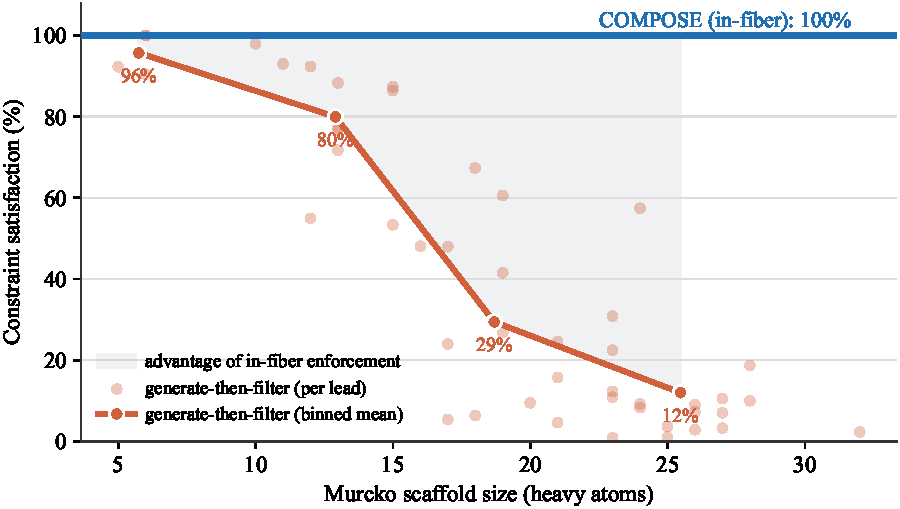
\includegraphics[width=0.74\textwidth]{figures/scaffold_collapse.pdf}
\caption{\textbf{Exact scaffold satisfaction versus generate-then-filter collapse.} Enforcing a fixed Murcko scaffold in the legal fiber holds \method at full satisfaction for every lead (blue), whereas drawing the same base model's proposals and filtering post hoc collapses monotonically with scaffold size (terracotta: per-lead points, binned means annotated). The shaded region is the widening advantage of in-fiber enforcement. Axis values are illustrative; frozen numbers are \XXX{} (\cref{tab:scaffold}).}
\label{fig:scaffold_collapse}
\end{figure}

\paragraph{Constraints conjoin freely in the fiber, multiplicatively for filtering (\cref{fig:conjunction}).}
Real specifications are conjunctions. As independent constraints---a similarity floor, the scaffold, forbidden motifs, and a molecular-weight/logP/QED box---are conjoined, generate-then-filter's usable yield falls multiplicatively to \ConjunctionFullSpec{} at the full spec, while in-fiber enforcement stays at \ComposeScaffoldSatisfaction{} because each constraint only prunes $\A(G)$. Restricted to the multi-property physicochemical box under an exact scaffold, per-sample joint satisfaction is \PhyschemBoxInFiber{} for \method vs.\ \PhyschemBoxBaseline{} for filtering (a \PhyschemBoxFactor{} gap), with the scaffold held at \ComposeScaffoldSatisfaction{}; we report the fair \emph{per-sample} joint rate, never a selected subset against an all-sample baseline.

\begin{figure}[t]
\centering
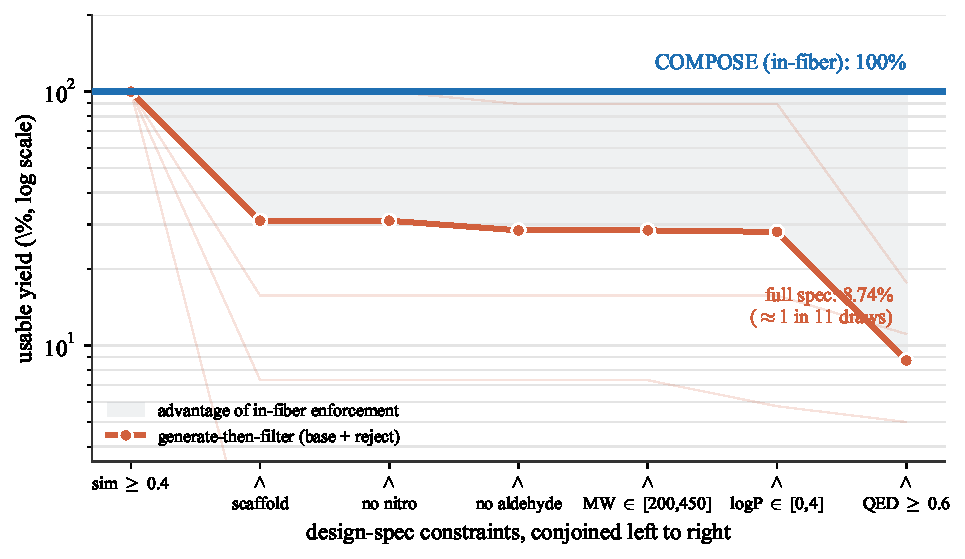
\includegraphics[width=0.82\textwidth]{figures/conjunction_funnel.pdf}
\caption{\textbf{Conjunctive design specs: in-fiber enforcement composes, filtering collapses.} Usable yield as design-spec constraints are conjoined left to right. \method (blue) stays at full yield because each constraint only prunes the legal fiber; generate-then-filter (terracotta) collapses multiplicatively to \ConjunctionFullSpec{} at the full spec. Numbers illustrative; frozen values \XXX.}
\label{fig:conjunction}
\end{figure}

\subsection{Oracle efficiency and anytime behaviour}
\label{sec:oracle}

Because feasibility is checked before scoring, every oracle call \method makes lands on a feasible candidate---\ComposeOracleEfficiency{} usable-oracle efficiency by construction. Generate-then-filter must score every candidate before discarding, so its efficiency equals its satisfaction fraction, \ComposeBaselineOracleEfficiency{} overall, leaving up to \ComposeBaselineOracleWastedHard{} of the budget wasted on the hardest scaffolds. This is a structural, not tuned, advantage on the very axis oracle-budgeted optimization is measured. Value-guided SMC over the rewrite CTMC with the scaffold enforced in the fiber improves QED on \ComposeConstrainedLeadsImproved{} leads (mean \ComposeConstrainedQEDFrom{}$\to$\ComposeConstrainedQEDTo{}, \ComposeConstrainedQEDGain{}) at \ComposeOracleEfficiency{} oracle efficiency while preserving the scaffold on every lead. Because every committed state is a usable molecule, the process is anytime (\cref{fig:anytime}): the median lead reaches $90\%$ of its final gain within \ComposeAnytimeCalls{} oracle calls, and sampling can be stopped, inspected, or resumed at any intermediate. We deliberately do \emph{not} run an unconstrained QED success-rate race: this controller is oracle-hungry and is not a matched comparison to oracle-light conditional models (\cref{sec:limits}); QED here is the objective inside a constrained task, not a leaderboard claim.

\begin{figure}[t]
\centering
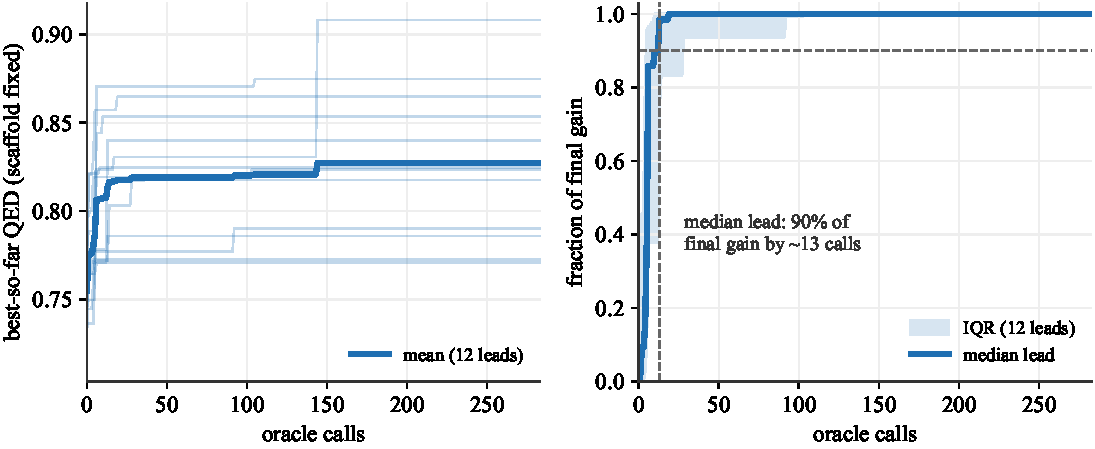
\includegraphics[width=\textwidth]{figures/anytime.pdf}
\caption{\textbf{Anytime constrained optimization.} With the Murcko scaffold enforced in the fiber, best-so-far feasible QED climbs quickly and plateaus, so every intermediate is a usable, improving candidate (left: per-lead traces with bold mean). Right: fraction of each lead's final gain versus oracle calls (median with interquartile band); the median lead reaches $90\%$ of its final gain within ${\sim}\ComposeAnytimeCalls{}$ oracle calls. Numbers illustrative; frozen values \XXX.}
\label{fig:anytime}
\end{figure}

\subsection{Exactness anchor: the Doob \texorpdfstring{$h$}{h}-transform}
\label{sec:exactness}

On an exhaustive \ComposeExactnessStates{}-state size-capped slice of the production legal-event CTMC, the Doob $h$-transform of the learned generator enforces a rule-closed target-set condition exactly (\cref{fig:doob}): the tilted one-step kernels reproduce the exact Bayes conditional endpoint to $\ell_\infty$ error \ComposeExactnessLinf{}, the tilted generator $Q^h$ is a valid generator (nonnegative off-diagonals, row sums zero to machine precision), and generator-level integration converges first-order to the exact conditional across conditioning predicates. This is the control law with $\Psi=h_t(H)/h_t(G)$, and it certifies the control interface where the harmonic function is tractable. A finite-particle controller using the exact twist reaches a target total variation with about \ExactHParticleFactor{} fewer particles than an untwisted bootstrap SMC (\cref{fig:doob}). In the full state space $h$ is intractable, so property conditioning uses the approximate value-guided SMC of \cref{sec:oracle}, and \cref{cor:endpoint} gives the endpoint law only under an exact model.

\begin{figure}[t]
\centering
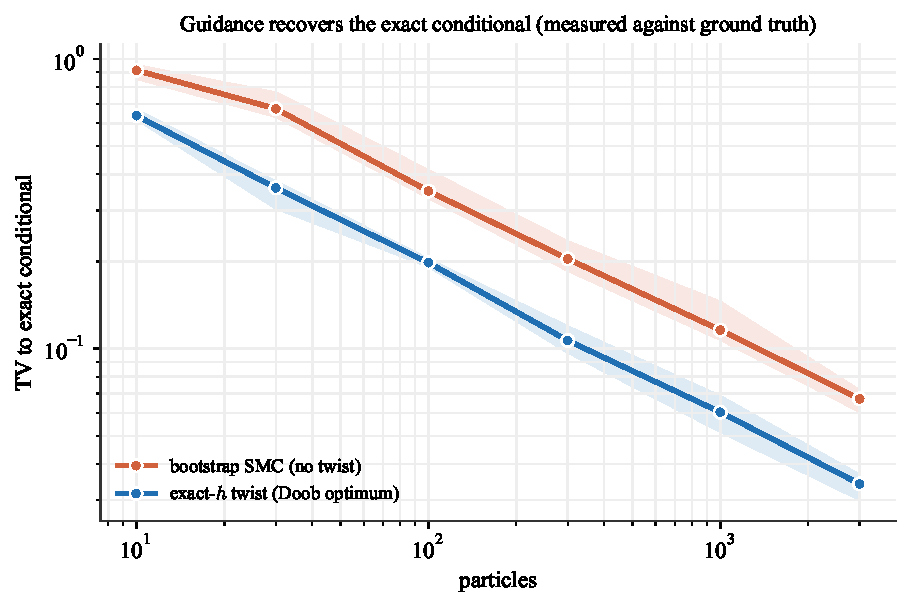
\includegraphics[width=0.72\textwidth]{figures/doob_guidance_ground_truth.pdf}
\caption{\textbf{Guidance recovers the exact conditional.} Total variation to the exact Bayes conditional versus particle count on the enumerated CTMC slice: the exact-$h$ (Doob-optimal) twist reaches a target TV with about \ExactHParticleFactor{} fewer particles than untwisted bootstrap SMC, and both converge. Curves are schematic; frozen values \XXX.}
\label{fig:doob}
\end{figure}

\subsection{De novo sufficiency and its honest limits}
\label{sec:denovo}

The de novo evaluation is the sufficiency gate for the substrate, not a distribution-learning leaderboard; validity is guaranteed by construction (\cref{prop:closure}) and we report the empirical rate only for completeness (\cref{tab:main}). \method is valid, unique, novel, and internally diverse, and its physicochemical descriptor marginals are reported as Wasserstein distances against a held-out reference. FCD is deferred to the final GuacaMol table (we do not stage an FCD arms race).

\begin{table}[t]
\centering
\caption{De novo sufficiency on GuacaMol (C/N/O/F): a sufficiency gate, not a distribution-learning leaderboard. FCD deferred to the final GuacaMol table. \method validity is guaranteed by construction (\cref{prop:closure}); the empirical rate is reported for completeness. Desc.\ $W_1$ is the mean physicochemical descriptor Wasserstein distance (logP, QED, MW, TPSA, rings). Baseline cells are to be run or cited; all values \XXX.}
\label{tab:main}
\small
\begin{tabular*}{\textwidth}{@{\extracolsep{\fill}}lcccccc}
\toprule
Method & Valid $\uparrow$ & Unique $\uparrow$ & Novel $\uparrow$ & Desc.\ $W_1\downarrow$ & Int.\ div.\ $\uparrow$ & Train cov.\ $\uparrow$\\
\midrule
DiGress & \XXX & \XXX & \XXX & \XXX & \XXX & \XXX\\
DeFoG & \XXX & \XXX & \XXX & \XXX & \XXX & \XXX\\
GrIDDD & \XXX & \XXX & \XXX & \XXX & \XXX & \XXX\\
Morph & \XXX & \XXX & \XXX & \XXX & \XXX & \XXX\\
\midrule
\method (base) & \ComposeValidity & \ComposeUniqueness & \ComposeNovelty & \ComposeDescriptorW & \ComposeDiversity & \ComposeCoverage\\
\method (ring-fix, planned) & \XXX & \XXX & \XXX & \XXX & \XXX & \XXX\\
\bottomrule
\end{tabular*}
\end{table}

\paragraph{Known ring-taxonomy defect (\cref{tab:ring}).}
The current base has a genuine flaw we do not paper over: it overproduces small (3--4-membered) rings and underproduces aromaticity relative to the reference (\cref{tab:ring})---exactly what the descriptor-Wasserstein column captures---so we do \emph{not} claim de novo state of the art. The cause is the ring factorization, and the fix (switching the rate factorization to a superposed head and the ring template to a hierarchical topology--cycle scheme, warm-started from the current base) is \emph{mechanism-proven} on a falsifier test but not yet trained at scale. \Cref{tab:ring} lists the reference, the current base, and the ring-fixed retrain target side by side.

\begin{table}[t]
\centering
\caption{Ring-taxonomy marginals (fraction of atoms/rings by class) against a held-out reference. The current base overproduces small rings and underproduces aromaticity---the known defect; the ring-fixed retrain is the target. All values \XXX.}
\label{tab:ring}
\small
\begin{tabular*}{\textwidth}{@{\extracolsep{\fill}}lcccccc}
\toprule
 & Small ring (3--4) & Aromatic frac. & Fused & Bridged & Spiro & Macrocycle\\
\midrule
Reference & \DenovoSmallRingRef & \DenovoAromaticRef & \XXX & \XXX & \XXX & \XXX\\
\method (base) & \DenovoSmallRing & \DenovoAromatic & \XXX & \XXX & \XXX & \XXX\\
\method (ring-fix, planned) & \XXX & \XXX & \XXX & \XXX & \XXX & \XXX\\
\bottomrule
\end{tabular*}
\end{table}

\begin{table}[t]
\centering
\caption{Path and structural fidelity across source priors/couplings. All-step metrics audit every accepted intermediate, not only endpoints; all values \XXX.}
\label{tab:path}
\small
\begin{tabular*}{\textwidth}{@{\extracolsep{\fill}}lccccccc}
\toprule
Variant & Step valid & Step conn. & Size TV & Cycle TV & Ring TV & Budget & Events\\
\midrule
Null prior & \XXX & \XXX & \XXX & \XXX & \XXX & \XXX & \XXX\\
Independent tree & \XXX & \XXX & \XXX & \XXX & \XXX & \XXX & \XXX\\
Size-matched Graft & \XXX & \XXX & \XXX & \XXX & \XXX & \XXX & \XXX\\
Flexible-size Graft & \ComposeTrajectoryValidity & \ComposeTrajectoryConnectivity & \ComposeSizeTV & \ComposeCycleRankTV & \ComposeRingSizeTV & \XXX & \ComposeMeanEvents\\
\bottomrule
\end{tabular*}
\end{table}

\subsection{Controller composition and the quotient}
\label{sec:composition}

The control law is sampler-agnostic: the same learned rates admit different $\Psi$ without retraining. We specify three controller instantiations and one representation ablation, run on the source-conditioned edit flow (\cref{sec:source-conditioned}) for the editing setting.

\paragraph{Controllers.}
(i) A \emph{MOG-style} tilt $\Psi=\exp\{\beta\,R(\Delta s(G,H)\cdot\omega)\}$ that ranks each canonical molecular successor's local improvement vector against a preference direction, optionally with a cone filter, lifted from token replacements to molecular successors. (ii) A \emph{Doob-lifted} controller $\Psi=h_t(H)/h_t(G)$ approximated by short rollouts, exact where enumerable (\cref{sec:exactness}). (iii) An \emph{archive-aware SMC} controller that scores and deduplicates canonical successors, adds them to a shared archive, and resamples by scalarized utility plus archive contribution. \Cref{tab:composition} reports each against the same-substrate uniform-legal proposal and a graph-GA reference at matched oracle budget.

\paragraph{Quotient vs.\ action-level guidance.}
\label{sec:ablate-quotient}
A representation-correct controller ranks canonical molecules $H$; an action-level controller ranks marked actions $a$ and so hands a molecule extra probability when it admits more syntactic derivations. We test this by duplicating rewrite lowerings (or exploiting symmetric molecules) and measuring whether the controlled molecular distribution is invariant: a quotient controller should be invariant to alias multiplicity, an action-level controller should drift. \Cref{tab:composition} includes this ablation and reports the measured divergence.

\begin{table}[t]
\centering
\caption{Controller composition and the quotient ablation, at matched oracle budget on the source-conditioned edit flow (\cref{sec:source-conditioned}). Alias TV is the total variation between controlled molecular distributions under duplicated lowerings (lower is better; a quotient controller should be invariant). All values \XXX.}
\label{tab:composition}
\small
\begin{tabular*}{\textwidth}{@{\extracolsep{\fill}}lcccc}
\toprule
Controller $\Psi$ & Feasible HV AUC $\uparrow$ & Unique ND $\uparrow$ & Acceptance $\uparrow$ & Alias TV $\downarrow$\\
\midrule
Uniform-legal (no learned rate) & \XXX & \XXX & \XXX & \XXX\\
Graph GA (task-level ref.) & \XXX & \XXX & \textemdash & \textemdash\\
MOG-style tilt & \XXX & \XXX & \XXX & \XXX\\
Doob-lifted & \XXX & \XXX & \XXX & \XXX\\
Archive-aware SMC & \XXX & \XXX & \XXX & \XXX\\
\midrule
Action-level guidance (ablation) & \XXX & \XXX & \XXX & \XXX\\
Quotient guidance (ours) & \XXX & \XXX & \XXX & \XXX\\
\bottomrule
\end{tabular*}
\end{table}

\subsection{Anytime Pareto-set editing: designed capability and future work}
\label{sec:editing}

The substrate's designed hero application is \emph{anytime Pareto-set editing}: because every visited state is a molecule, the output of a trajectory is not one endpoint but its source-relative nondominated archive $A_{k+1}=\mathrm{ND}(A_k\cup\{G_{k+1}\})$, and the path-level objective is $U(\tau)=\mathrm{HV}(A_T)-\lambda\,\mathrm{EditCost}(\tau)$. Every scored intermediate can enter the archive, seed a branch, be reused under a different preference, or be cached across particles by canonical identity. The principled controller augments the state with the archive, $Z_t=(G_t,A_t)$, and applies a Doob transform for the path utility $U(A_T)$; a first implementation is the archive-aware SMC of \cref{sec:composition} with preference vectors adapted toward under-covered archive regions (Pareto continuation). Because restart points are molecules, rotating $\omega$ needs no re-noising or re-decoding.

\paragraph{Why this is future work, not a present result.}
A fair editing win requires the source-conditioned edit flow (\cref{sec:source-conditioned}); the released de novo prior is out of distribution as a \emph{starting} state at a real lead. We therefore specify the experiment fully and leave its results \XXX{} by design (\cref{tab:editing}). The protocol initializes from held-out CNOF leads with $\ge 3$ conflicting objectives, runs each controller and an endpoint-only ablation at matched oracle budget with canonical caching, and reports feasible-hypervolume AUC, unique nondominated molecules, frontier coverage, source edit distance, structural retention, and all-state validity. The decisive comparisons are (a) all-visited-state archive vs.\ endpoint-only archive at identical oracle calls---does the path itself add value?---and (b) learned quotient rates vs.\ uniform-legal proposals---does the learned generator matter? This experiment also resolves the frontier-recovery \emph{efficiency} question left open in \cref{sec:mechanism}.

\begin{table}[t]
\centering
\caption{Anytime Pareto-set editing (specified; requires the source-conditioned edit flow of \cref{sec:source-conditioned}). Source-relative multi-objective editing from held-out CNOF leads with $\ge 3$ conflicting objectives at matched oracle budget. All values \XXX{} by design---this is the paper's planned hero experiment, not a completed result.}
\label{tab:editing}
\small
\begin{tabular*}{\textwidth}{@{\extracolsep{\fill}}lcccccc}
\toprule
Method & Feas.\ HV AUC $\uparrow$ & Unique ND $\uparrow$ & Frontier cov.\ $\uparrow$ & Src.\ edit dist. & Retention $\uparrow$ & All-state valid $\uparrow$\\
\midrule
Endpoint-only (ablation) & \EditFeasibleHV & \EditUniqueND & \EditFrontierCoverage & \EditSourceDistance & \EditRetention & \XXX\\
Uniform-legal archive & \XXX & \XXX & \XXX & \XXX & \XXX & \XXX\\
MARS / MIMOSA (task-level) & \XXX & \XXX & \XXX & \XXX & \XXX & \XXX\\
Graph GA (task-level) & \XXX & \XXX & \XXX & \XXX & \XXX & \XXX\\
\method anytime archive (ours) & \EditFeasibleHV & \EditUniqueND & \EditFrontierCoverage & \EditSourceDistance & \EditRetention & \XXX\\
\bottomrule
\end{tabular*}
\end{table}

\subsection{Ablations and process diagnostics}
\label{sec:ablations}

Three ablations isolate which parts of the construction carry the behaviour. \emph{Learned vs.\ uniform-legal:} replace $Q_\theta$ by the uniform legal rate under the same controller, testing whether Generator Matching contributes beyond a valid edit graph. \emph{Substrate vs.\ token/ambient:} run the same MOG-/AReUReDi-style controller on \method and on a SMILES-token or ambient-graph base, testing whether the molecular substrate matters. \emph{Quotient vs.\ action-level} (\cref{sec:ablate-quotient}). \Cref{tab:ablations} additionally isolates the prior/coupling, Graft, ring macros, alias aggregation, and importance stratification on de novo fidelity.

\begin{table}[t]
\centering
\caption{Matched ablations isolating which construction choices produce the observed behaviour. Path length is measured on compiled teachers; descriptor $W_1$ and ring-size TV on target-free learned samples. All values \XXX.}
\label{tab:ablations}
\small
\begin{tabular}{lccc}
\toprule
Variant & Desc.\ $W_1\downarrow$ & Mean teacher length $\downarrow$ & Ring-size TV $\downarrow$\\
\midrule
Null source & \NullPriorFCD & \XXX & \XXX\\
Primitive tree (delete/regrow) & \PrimitiveTreeFCD & \XXX & \XXX\\
Tree + Graft & \GraftTreeFCD & \ComposePathLength & \XXX\\
No coordinated ring macros & \NoMacroFCD & \XXX & \XXX\\
No successor alias aggregation & \NoAliasFCD & \XXX & \XXX\\
No importance-correct stratification & \NoStratificationFCD & \XXX & \XXX\\
\bottomrule
\end{tabular}
\end{table}

Reachability alone does not establish learned capability. We therefore report event fractions for Graft (\ComposeGraftFraction), grow (\ComposeGrowFraction), shrink (\ComposeShrinkFraction), retype (\ComposeRetypeFraction), and ring events (\ComposeRingFraction), stratified by model time and source/endpoint size, and measure whether source edges survive, whether paths visit the one-atom state, and whether samples show the covariance collapse that aggregate FCD can obscure.

\subsection{Developmental evidence is not a benchmark result}
\label{sec:dev}

Current engineering evidence establishes executability, not final quality. In a developmental size-matched Graft run the compiler produced \XXX{} supported programs for \XXX{} of \XXX{} targets; a checkpoint reduced held-out RGM loss from \XXX{} to \XXX{} and reached \XXX{} teacher family accuracy; an early sampling gate produced \XXX{} valid/connected accepted rollouts on its restricted chemistry. These values diagnose the implementation and motivate the confirmatory experiments. They are not directly comparable to full GuacaMol baselines, are not inserted into \cref{tab:main,tab:ablations}, and will be replaced by frozen multi-seed results.

\section{Discussion and Limitations}
\label{sec:limits}

\paragraph{The contribution and what it is not.}
The contribution is a control-closed molecular substrate: rewriting defines a valid state graph and executable event semantics, Generator Matching learns how probability flows on it, and the control law~\eqref{eq:control-law} lets any controller reweight the same molecular rates without leaving $\M$ (\cref{prop:control-closure}). The empirical spotlight is that Pareto reachability depends on path topology---only well-posed because intermediates are molecules---with structural control, oracle efficiency, and the Doob exactness anchor as supporting evidence. We are deliberate about what this is \emph{not}. We do not claim to out-optimize strong task-level search: a graph genetic algorithm and PMO-style methods are strong molecular optimizers \citep{jensen2019graphga,gao2022pmo}, and uniform-legal search over the same edit graph is itself a strong controller. Our claim is the substrate and its mechanism, and the learned rate must justify itself against uniform-legal (\cref{sec:composition,sec:ablations}), not against a GA leaderboard.

\paragraph{Editing is out of distribution for a de novo prior.}
The released model is a universal edit prior trained from carbon-tree trajectories, so dropping it at a real lead and asking it to edit is off-distribution as a \emph{starting} state. The anytime-Pareto-editing hero (\cref{sec:editing}) and the learned-vs-uniform efficiency study therefore require the source-conditioned edit flow (\cref{sec:source-conditioned}); we specify them fully and leave their results \XXX. Relatedly, the frontier-recovery \emph{efficiency} claim is undecided: we establish that greedy control has a structural ceiling and that valid detours cross it, but whether detours recover the frontier at matched oracle budget is left open.

\paragraph{The de novo base has a ring defect.}
The current base overproduces small rings and underproduces aromaticity (\cref{tab:ring}); we do not claim de novo state of the art, and the fix is mechanism-proven but untrained at scale. Our oracle-guided SMC is also oracle-hungry and is not a matched comparison to oracle-light conditional models; a learned oracle-light route (classifier-free conditioning, reward fine-tuning) remains weak and is future work. QED is reported only inside constrained tasks or as a $\Psi$-steering demonstration, never as a standalone leaderboard.

\paragraph{Scope of the closure guarantee.}
The declared domain is connected, valence-admissible 2D molecular graphs with implicit hydrogens. This is \emph{molecular-state} closure, not comprehensive chemical feasibility: it does not guarantee synthesizability, 3D plausibility, stereochemistry, or oracle reliability, and a rewrite trajectory is not a synthesis route, so all-step molecular validity is closure of the design space rather than physical synthesizability. Stereochemistry, conformers, radicals, metals, and multi-center bonding need extensions; a finite typed ring catalog can under-cover rare programs; and the compiler introduces inductive bias by concentrating supervision on one of many valid paths.

\paragraph{Comparisons to verify.}
Our characterizations of external controllers and editors (MOG-DFM, AReUReDi, pCoMole, MARS, MIMOSA) originate in a strategy memo and are treated as claims to verify against primary sources before any head-to-head result; the already-verified ConStruct/PRODIGY/CoCoGraph positioning is stated as fact and the remainder as to-check. Hard support guarantees do not imply low FCD, likelihood optimality, rapid mixing, or chemical usefulness.

\section{Conclusion}

\method turns stochastic molecular graph rewriting into the transition substrate of a learned generative process whose states are always molecules. Endpoint-conditioned valid programs provide exact jump-rate targets; Generator Matching removes the endpoint and program; the quotient puts probability on canonical molecular successors; and guarded execution keeps every committed state in the declared space. The consequence is closure under control: one control law composes hard requirements, preference tilts, Doob transforms, SMC, and MH on the same rates without retraining. On exact rewrite graphs this substrate exposes a mechanism---Pareto reachability depends on path topology, so greedy control has a structural ceiling that valid molecular detours cross---and it supports structural control, oracle efficiency, and an exactness anchor. Its designed hero, anytime Pareto-set editing, and the source-conditioned edit flow it requires are specified and left as the immediate next step. Every empirical value in this draft is a placeholder (\XXX) pending frozen artifacts.

\bibliography{references}
\bibliographystyle{iclr2026_conference}

\appendix

\section{Operator Semantics and Contracts}\label{app:operators}

For each $r$, $\Match_r(G)$ is the finite set of pattern monomorphisms satisfying structural application conditions. The payload $\xi$ contains new atom/bond states or a macro program. Rule, match, and payload define a partial map $\T_{r,m,\xi}:\M\rightharpoonup\M$. The implementation follows a propose--validate--commit discipline: construct a candidate copy, update implicit hydrogens and bond states jointly, run local valence and global sanitization/connectivity checks, then commit or expose no transition.

\begin{table}[h]
\centering
\caption{Minimum application conditions. The implementation may impose additional grammar-specific checks.}
\small
\begin{tabularx}{\textwidth}{lX X}
\toprule
Rule & Structural condition & Chemical/transaction condition\\
\midrule
Atom insert & empty slot; occupied anchor & allowed atom/bond; endpoint valences feasible\\
Atom delete & removable atom; remainder connected & neighbor H compensation; sanitized successor\\
Atom restate & occupied slot & joint element/charge/H state allowed\\
Bond insert & absent edge; endpoints occupied & allowed order; valence feasible; nonidentity\\
Bond delete & existing non-bridge edge & endpoint H compensation; sanitized successor\\
Bond reorder & existing edge & joint order/H update feasible\\
Subtree Graft & old edge is a bridge; new endpoints cross its cut & atomic cut+attach; all endpoint valences feasible\\
Ring ear insert & valid anchors and fresh internal slots & joint typed path closes; full lowering replays\\
Ring ear delete & matched removable ear; remainder connected & exact inverse payload; full lowering replays\\
Ring restate & fixed matched cyclic system & coordinated atom/bond state passes executor\\
\bottomrule
\end{tabularx}
\end{table}

\paragraph{Why macros remain rewrite events.}
A macro has one chemically interpretable successor and one learned rate. Its lowering is a proof-carrying implementation artifact: each micro state must also lie in $\M$, but inference exposes the macro as one marked CTMC event. This avoids treating arbitrary edit bundles as simultaneous jumps. Unrelated micro events may conflict on valence, fail to commute, and create an exponential bundle space; only verified compound semantics are promoted.

\paragraph{Ring topology coverage.}
Every 2-connected simple graph admits an open-ear decomposition starting from a cycle. Consequently, root/attached cycles plus distinct-anchor ears span biconnected cyclic topology at the graph level. Spiro systems join blocks at an articulation and are represented by same-anchor cycles. Repeated composition covers fused, bridged, spiro, linked, and mixed polycycles. Chemical feasibility remains enforced per typed payload; the graph theorem does not certify strain or synthesis.

\section{Source Priors and Couplings}\label{app:prior}

\subsection{Degree-bounded carbon-tree sampler}

Given size law $\mu$ on $\{1,\ldots,N_{\max}\}$:
\begin{enumerate}[leftmargin=*]
    \item sample $N\sim\mu$;
    \item sample a Pr\"ufer sequence with rejection or capped construction so every degree is at most four;
    \item decode the tree, assign neutral carbon atom states and single bonds, and derive implicit hydrogens;
    \item assert connectivity, valence validity, and the declared slot count.
\end{enumerate}
The source sampler consumes only $\mu$ and an RNG seed. For a training pair, the tree draw is independent of the endpoint conditional on the selected source size.

\subsection{Stationary size jitter}

Let $J$ be a Markov kernel on sizes with stationary law $\mu$. Drawing $N_1\sim\mu$ then $N_0\sim J(\cdot\mid N_1)$ preserves the source marginal:
\begin{equation}
\Pr(N_0=m)=\sum_n\mu(n)J(m\mid n)=\mu(m).
\end{equation}
A local proposal $n\to n\pm1$ with a Metropolis--Hastings accept/reject correction is a simple reversible choice. The jitter scale controls teacher transport cost but must not be confused with the source law. At inference, $N_0$ is drawn directly from $\mu$ without sampling a target size.

\section{Program Compilation Algorithms}\label{app:compiler}

\subsection{Primitive connectivity-preserving transport}

For completeness, any source can be reduced topologically to one retained atom: delete non-tree edges to expose a spanning tree, then remove leaves. Reverse the construction for a target spanning tree, add chords, and apply typed restatements. The production compiler uses direct common structure and Grafts because the one-atom route is valid but statistically wasteful.

\subsection{Graft transport}

Given equal-order carbon tree $T_0$ and target $G_1$:
\begin{enumerate}[leftmargin=*]
    \item align temporary source slots with target slots and choose a spanning tree $T_1\subseteq G_1$ maximizing $|E(T_0)\cap E(T_1)|$;
    \item while $T\neq T_1$, select $e\in E(T_1)\setminus E(T)$; adding $e$ creates a unique cycle, from which select $f\in E(T)\setminus E(T_1)$; execute the corresponding atomic subtree Graft and validate;
    \item restate retained atom states and tree-bond classes in a guard-feasible order;
    \item install target chords with verified ring-ear or bond events;
    \item canonicalize and assert exact equality with $G_1$; replay the complete program independently.
\end{enumerate}
The graph-level edge-exchange loop performs at most $(n-1)-|E(T_0)\cap E(T_1)|$ iterations. Chemistry guards may reject a nominal exchange, so the implementation searches alternative cycle edges and uses a constructive fallback. A compilation failure is explicit; it is never converted to a truncated target.

\subsection{Ring catalog construction}\label{app:ring-catalog}

The current finite proposal catalog is mined only from training programs:
\begin{enumerate}[leftmargin=*]
    \item decompose each target into biconnected blocks and its block--cut tree;
    \item compile cyclic blocks into root/attached cycles, open ears, same-anchor cycles, and electronic restatements;
    \item canonicalize marks modulo slot permutation and chemically equivalent aliases;
    \item count marks and retain a declared training-only vocabulary or factorized fields;
    \item audit full-program coverage independently on train, validation, and test.
\end{enumerate}
Frequency initializes or stratifies learning but does not define structural legality. The final factorized decoder predicts family, anchors, span, and typed atom/bond payload so that uncommon combinations need not occur as memorized fragments.

\subsection{Program-cache reproducibility}

Programs are stored as rewrite instructions plus byte-packed exact graph checkpoints rather than a dense graph at every progress position. A sampled state replays at most $c-1$ validated actions from the nearest checkpoint. CPU compilation writes atomic, signature-validated shards with a manifest containing split hashes, compiler version, chemistry grammar, prior/coupling configuration, ring catalog hash, seeds, and checkpoint interval. A GPU training stage refuses to start from an incomplete cache. These choices change throughput and storage, not the mathematical path distribution.

\section{Proofs}\label{app:proofs}

\subsection{Proof of \cref{prop:closure}}

Induct on committed events. The base state is in $\M$. If $G_n\in\M$, the CTMC has support only on $a\in\A(G_n)$; by \eqref{eq:legal-fiber}, $G_{n+1}=\T_aG_n\in\M$. Local boundedness excludes explosion on the finite horizon, so only finitely many jumps occur almost surely. The conclusion applies equally to teacher programs and learned sampling because both invoke the same executor. \qed

\subsection{Proof of \cref{prop:control-closure}}

By \eqref{eq:quotient-rate} the learned generator has support only on $\Sset(G)\subseteq\M$. The control law~\eqref{eq:control-law} sets $\widetilde Q_t(G,H)=\one\{C(H)\}\,Q_{\theta,t}(G,H)\,\Psi_t(G,H,\omega)$, which is a nonnegative pointwise product; it vanishes whenever $Q_{\theta,t}(G,H)=0$, hence whenever $H\notin\Sset(G)$. So the controlled chain jumps only to $H\in\Sset(G)\subseteq\M$, and the induction of \cref{prop:closure}---which uses only that every jump lands in $\M$ under the same executor---applies verbatim, giving closure almost surely on the finite horizon. If $C\equiv1$ and $\Psi_t>0$ on $\Sset(G)$, then $\widetilde Q_t(G,H)>0 \iff Q_{\theta,t}(G,H)>0$, so the two generators have identical support. Neither factor can create a transition to an $H\notin\Sset(G)$, since both multiply the learned rate. \qed

\subsection{Proof of \cref{prop:barrier}}

If $H$ is reachable by a $U_\omega$-nondecreasing valid path $\tau$, then $U_\omega(G_k)\ge U_\omega(G_s)$ at every step, so $\max_k[U_\omega(G_s)-U_\omega(G_k)]_+=0$ along $\tau$ and hence $B_\omega(H)=0$ by minimality. Conversely, if $B_\omega(H)=0$ the minimizing path $\tau$ has $\max_k[U_\omega(G_s)-U_\omega(G_k)]_+=0$, i.e.\ $U_\omega(G_k)\ge U_\omega(G_s)$ for all $k$; such a path never drops below the source utility, and (restricting to the achieved values) is nondecreasing in the scalarization sense used by a monotone controller. Thus the monotone-reachable set is exactly $\{H:B_\omega(H)=0\}$. Every $H$ in the connected component of $G_s$ is reachable by \emph{some} valid path (\cref{prop:reachability} at the topological level, and by compiler-certified chemistry in practice), so the detour-reachable set is that whole component; its difference with the zero-barrier set is $\{H:B_\omega(H)>0\}$, unreachable by any monotone path yet reachable by a detour. \qed

\subsection{Proof of \cref{prop:reachability}}

For connected $G$, choose a spanning tree $T_G$. Delete every edge in $E(G)\setminus E(T_G)$; each is on a cycle at deletion and is therefore not a bridge, so connectivity is preserved. Repeatedly delete leaves until one vertex remains. From one vertex, reverse leaf insertions to construct a spanning tree $T_H$ of $H$, then insert edges in $E(H)\setminus E(T_H)$. Every intermediate is connected.

For aligned trees $T$ and $T_1$, take $e\in E(T_1)\setminus E(T)$. Adding $e$ creates a unique cycle. That cycle contains an edge $f\in E(T)\setminus E(T_1)$; otherwise $T_1$ would contain a cycle. Replacing $f$ by $e$ is one subtree Graft, preserves the tree property, and increases overlap with $T_1$ by one. Repetition terminates after at most $(n-1)-|E(T_0)\cap E(T_1)|$ exchanges. \qed

\subsection{Proof of \cref{prop:gm}}

Fix occupied $(G,t,H)$ and let $Y=R_t^Z(H\mid X_t,K_t)$ conditional on $X_t=G$. The part of \eqref{eq:gm-objective} depending on scalar prediction $u\ge0$ is
\begin{equation}
\ell(u)=u-\E[Y\mid X_t=G]\log u,
\end{equation}
with target-only terms omitted. For $u>0$, $\ell'(u)=1-\E[Y\mid X_t=G]/u$ and $\ell''(u)=\E[Y\mid X_t=G]/u^2\ge0$. If the mean is positive, the unique minimizer is its value; if zero, the infimum is attained at $u=0$ by continuity. Finite sums commute with conditional expectation, so the result applies after alias aggregation. \qed

\subsection{Proof of \cref{cor:endpoint}}

The program mixture induces marginal law $p_t$ satisfying the Kolmogorov forward equation with $Q_t$ from \eqref{eq:marginal-generator}; this is the standard conditional-to-marginal Generator Matching identity. Under \cref{ass:finite}, the finite-state forward equation has a unique solution. If $Q_{\theta,t}=Q_t$ and both laws begin at $\pzero$, their marginals agree for all $t$. By \cref{ass:path}, the program mixture terminates at $\pdata$, hence so does the exact learned process. \qed

\subsection{Importance-correct progress stratification}

Let $p(k\mid t,Z)$ be the binomial progress law and $h(k\mid Z)$ a family-balanced proposal. Sample from $\widetilde p=(1-\rho)p+\rho h$ and weight by $w=p/\widetilde p$. For any integrable per-progress loss $g$, $\E_{\widetilde p}[wg]=\sum_kp(k)g(k)=\E_p[g]$. Since $\widetilde p\ge(1-\rho)p$, support is retained for $\rho<1$.

\section{Model, Training, and Sampling Details}\label{app:model}

\subsection{Neural architecture}

The graph encoder embeds atom type, formal charge, implicit hydrogen count, bond class, model time, and ring/topology context. Message passing produces node and graph representations. A graph head predicts total hazard; a masked family head predicts the rule schema; atom, pair, and template heads predict operands and typed payloads. Hierarchical normalization prevents a family with many raw matches from receiving probability solely because of multiplicity. The reported base uses hidden width $256$, $6$ message-passing layers, \ComposeParameters{} parameters, batch size $64$, the AdamW optimizer with decoupled weight decay $10^{-5}$, learning rate $3\times10^{-4}$ with $500$ warm-up steps, the linear schedule $\alpha(t)=t$ under operational time, and $1{,}000$ training updates of a $3{,}000$-step schedule (selected by held-out RGM loss). Final frozen-model values will be reported at full training.

\subsection{Training estimator}

For each minibatch item:
\begin{enumerate}[leftmargin=*]
    \item draw or load $(G_0,G_1,Z)$ from the declared coupling and compiled cache;
    \item sample time $t$ and progress $k$, optionally from the importance-correct stratified proposal;
    \item reconstruct $X_t=G_k^Z$ from its nearest packed checkpoint;
    \item encode $X_t$ once, form analytic legality masks, and evaluate \eqref{eq:gm-objective};
    \item aggregate aliases for the teacher successor and update $\theta$.
\end{enumerate}
We log hazard, family/operand accuracy, illegal-mask disagreements, gradient norm, and held-out RGM loss. Model selection uses a declared validation criterion without test FCD.

\subsection{Exact ancestral sampler}\label{app:sampler}

Let $0=s_0<\cdots<s_J=S$ be the operational-time grid. Starting from $G\sim\pzero$, at grid interval $j$:
\begin{enumerate}[leftmargin=*]
    \item compute $\lambda=\lambda_\theta(G,s)$ and masked marked probabilities;
    \item if $\lambda=0$, advance to $s_{j+1}$ and log a stall;
    \item otherwise draw $\Delta\sim\mathrm{Exponential}(\lambda)$;
    \item if $s+\Delta\ge s_{j+1}$, set $s=s_{j+1}$ without an event;
    \item else sample $a$ hierarchically, execute $G\leftarrow\T_aG$, set $s\leftarrow s+\Delta$, and recompute all rates.
\end{enumerate}
The event budget is a numerical safeguard and its hit rate is reported. There is no rejection loop over invalid actions: analytic masks and the executor define zero support, and any disagreement is an auditable implementation error.

\subsection{Complexity}

Let $n\le N_{\max}$, $d$ be hidden width, $L$ message-passing layers, and $C_r(G)$ the tensorized candidate count for family $r$. One rate evaluation costs the graph encoder plus masked heads, approximately $O(L(n d^2+|E|d)+\sum_r C_r(G)d)$ for the dense implementation, rather than one graph encoding per canonical successor. Compilation is offline and program-dependent; Graft tree alignment is polynomial and each edge exchange is validated. Final measured preprocessing time, peak memory, train throughput, and sample throughput are \ComposeTrainHours, \ComposePeakMemory, \XXX, and \ComposeThroughput.

\section{Complete Experimental Protocol}\label{app:experiments}

\subsection{Frozen data contract}

We will release raw input hashes, canonicalization code, exact accepted SMILES, split indices, $N_{\max}$, element/charge/bond vocabularies, every exclusion count, and the ring-catalog audit. Test molecules do not influence the source-size law, templates, hyperparameters, or checkpoint selection.

\subsection{FCD contract}

FCD is computed with one frozen ChemNet implementation and environment. Invalid or null samples are not replaced. We report generated/reference counts, total FCD, additive mean and covariance terms, generated/reference covariance traces, multi-seed mean and standard deviation, and bootstrap intervals. We use at least \XXX independent samples per final seed; any 2,000-sample diagnostic is labeled preliminary.

\subsection{Ablation protocols}

\paragraph{Prior/coupling.}
Hold architecture, data, steps, and sampler fixed; compare null, independently sized carbon tree, size-matched tree, and stationary size-jitter. Report teacher length as well as learned endpoint metrics.

\paragraph{Graft.}
Compare primitive delete/regrow transport with Graft-enabled transport on identical sampled source--target pairs. Measure compilation success, path length, one-atom visits, source-edge survival, training throughput, event use, and endpoint FCD/topology.

\paragraph{Rings.}
Compare scalar bond construction, topology-only ears, typed ears, and typed ears plus ring-system restatement. Report per-class recall/TV for aromatic, saturated, fused, bridged, spiro, small rings (3--4), ordinary rings (5--7), and macrocycles under the dataset definition.

\paragraph{Objective and quotient.}
Ablate total-hazard learning, importance-correct stratification, and canonical alias aggregation. The last ablation tests whether symmetric syntactic multiplicity biases chemical successor rates.

\subsection{Trajectory audits}

For every sampled event we record time, rule family, operands, pre/post canonical keys, hazard, and validity/connectivity flags. Aggregates include:
\begin{itemize}[leftmargin=*]
    \item rule-family and inverse-pair utilization by time and size;
    \item source-edge survival, topology edit distance, and one-atom-state visitation;
    \item ring class before and after every cyclic event;
    \item aliases per successor and marked-versus-quotient calibration;
    \item event-budget exhaustion, zero-hazard stalls, and time-grid sensitivity;
    \item agreement of analytic masks/direct sampling with exhaustive fibers on small graphs.
\end{itemize}

\subsection{Additional pending results}

\begin{table}[h]
\centering
\caption{Ring taxonomy distribution distances; all values pending.}
\small
\begin{tabular}{lcccccc}
\toprule
Method & Aromatic & Saturated & Fused & Bridged & Spiro & Macrocycle\\
\midrule
DiGress & XXX & XXX & XXX & XXX & XXX & XXX\\
Morph & XXX & XXX & XXX & XXX & XXX & XXX\\
\method & XXX & XXX & XXX & XXX & XXX & XXX\\
\bottomrule
\end{tabular}
\end{table}

\begin{table}[h]
\centering
\caption{Compute and storage; preprocessing is included and all values are pending.}
\small
\begin{tabular}{lccccc}
\toprule
Method & Parameters & Compile h & Train h & Peak memory & Molecules/s\\
\midrule
\method & \ComposeParameters & XXX & \ComposeTrainHours & \ComposePeakMemory & \ComposeThroughput\\
\bottomrule
\end{tabular}
\end{table}

\subsection{Controlled-design and editing protocol}

Structural control and source-relative editing are supporting and future thrusts of the substrate (\cref{sec:structural,sec:editing}). We initialize from held-out CNOF leads, optionally freeze a scaffold or SMARTS motif by removing incompatible actions from $\A(G)$, and evaluate constraint satisfaction, generate-then-filter usable fraction by hardness and by number of conjoined constraints, usable-oracle efficiency, constrained property gain, scaffold retention, anytime best-so-far reward, source edit distance, diversity, and all-step validity. The scaffold-retention, property-gain, and constraint-satisfaction values are \ComposeScaffoldRetention{}, \ComposePropertyGain{}, and \ComposeScaffoldSatisfaction{}. The anytime Pareto-set editing protocol (\cref{sec:editing}) runs on the source-conditioned edit flow (\cref{sec:source-conditioned}) and additionally reports feasible-hypervolume AUC versus oracle calls, unique nondominated molecules, frontier coverage, and canonical cache hit rate; its results are \XXX{} pending that model. The separate unconstrained oracle-hungry success rate (\ComposeConditionalSuccess{}) is reported only in this appendix with disclosed oracle budget and search-method comparators, never as a headline. Reward fine-tuning or inference guidance is reported separately from the unguided generator.

\section{Failure Modes, Broader Impact, and Reproducibility}

\paragraph{Failure modes.}
We stratify failures into compiler support, proposal-mask false negatives, executor discrepancies, zero-hazard stalls, event-budget exhaustion, source-memory artifacts, invalid ring electronics, over-fusion, macrocycle excess, and endpoint distribution mismatch. Chemical examples are selected by predeclared strata rather than only visual appeal.

\paragraph{Broader impact.}
The model can generate valid but unsafe, toxic, or controlled compounds. A distribution-learning score is not evidence of therapeutic value. Downstream property guidance requires access control, dual-use review, toxicity assessment, and wet-lab governance. Corpus bias and cheminformatics blind spots remain even when formal validity is guaranteed.

\paragraph{Artifact checklist.}
The final release will contain:
\begin{itemize}[leftmargin=*]
    \item code version, environment lockfile, and RDKit/ChemNet versions: \XXX;
    \item dataset, split, vocabulary, and canonicalization hashes: \XXX;
    \item all hyperparameters, seeds, source draws, and coupling settings: \XXX;
    \item compiled-program manifest, ring catalog, and recovery checkpoints: \XXX;
    \item generated SMILES, per-event trajectories, and raw metric outputs: \XXX;
    \item multi-seed summaries, confidence intervals, and failed-run disclosure: \XXX.
\end{itemize}

\section{Large Language Model Usage Statement}

Large language models were used for drafting and code assistance. All mathematical claims, citations, implementation details, and empirical values require author verification. No generated reference or result is retained without checking a primary source or frozen experiment artifact.

\end{document}
